\documentclass[9pt]{beamer}


\def\Title{Bayesian machine learning\\\vspace{3mm}
Bayesian deep learning}

\usetheme[height=0mm]{Rochester}
\usecolortheme{}
\usefonttheme[onlylarge]{structurebold}
\setbeamerfont*{frametitle}{size=\normalsize,series=\bfseries}
\setbeamertemplate{navigation symbols}{}
\setbeamercovered{dynamic}
\setbeamertemplate{itemize item}[triangle]
\setbeamertemplate{itemize subitem}[triangle]

%  use Darmstadt if commenting the next line
\usepackage[footheight=1em]{beamerthemeboxes}
\usepackage[natbib=true,backend=biber,citestyle=authoryear,maxbibnames=2]{biblatex}
\bibliography{../bib/biblio_julyan} % ../bib/stats,../bib/statsjulyan,../bib/learningjulyan

%\let\oldcite=\cite
%\renewcommand\cite[1]{\hyperlink{#1}{\textcolor{gray}{\oldcite{#1}}}}
%\let\oldcite=\citet
%\renewcommand\citet[1]{\hyperlink{#1}{\textcolor{gray}{\oldcite{#1}}}}
%\let\oldcitep=\citep
%\renewcommand\citep[1]{\hyperlink{#1}{\textcolor{gray}{\oldcitep{#1}}}}

\usepackage{amsmath,amssymb,amsthm,bbm}             % AMS Math
\usepackage[utf8]{inputenc}
\usepackage[english]{babel}
%\usepackage{myAlgorithm}
\usepackage{xcolor}
\usepackage{graphicx}
\usepackage{subfigure}
\usepackage{hyperref}
\usepackage{mathtools}
\usepackage{mathrsfs}
\usepackage{animate}
%\usepackage{fontawesome5} % twitter bird


\usepackage{color}
%\usepackage[citecolor=blue]{hyperref}
%\RequirePackage[citecolor=blue]{hyperref}
%\usepackage{animate}
\usepackage{xspace}
\usepackage{algorithm, algorithmic}
\usepackage{mathrsfs,dsfont}
\usepackage{amssymb,amsmath,amsthm,graphicx}
\usepackage{animate}
%\graphicspath{{./Figures/}}
\usepackage{setspace} % with \setstretch{1.3}
\usepackage{yfonts}
%\usepackage[square]{natbib}
%\usepackage{graphicx}

% packages on graphs and tables
\usepackage{booktabs}
\setlength{\heavyrulewidth}{1.5pt}
\setlength{\abovetopsep}{4pt}
\usepackage{rotating} % for tables


\usepackage{marvosym} % for website symbols
\usepackage{transparent}

\usepackage{appendixnumberbeamer} 

\usepackage{amsmath,amsthm}

\usepackage[export]{adjustbox}



\newtheorem{proposition}{Proposition}
\newtheorem{remark}{Remark}


\definecolor{forestgreen}{rgb}{0.13, 0.55, 0.13}
\definecolor{darkblue}{rgb}{0.0, 0.0, 0.65}
\definecolor{violet2}{rgb}{0.5,0,0.5}
\definecolor{orange2}{rgb}{0.8, 0.1, 0.1}       
\definecolor{red2}{rgb}{1, 0.4, 0}

\hypersetup{
	colorlinks=true,
	urlcolor=orange2,
	citecolor=orange2,
	linktoc=all,
	linkcolor=orange2}

\allowdisplaybreaks
%\renewcommand{\alert}[1]{\textcolor{red2}{#1}}
\newcommand{\question}[1]{\textcolor{forestgreen}{#1}}



\setbeamertemplate{footline}[frame number]


%%%%%%%%%%%%%%%%%
% see option in Beamer guide, section 10: https://tug.ctan.org/macros/latex/contrib/beamer/doc/beameruserguide.pdf
\AtBeginSection[] % Do nothing for \section*
{
\begin{frame}
\frametitle{Outline}
\tableofcontents[currentsection,
				 hideothersubsections]
\end{frame}
}


\AtBeginSubsection[] % Do nothing for \section*
{
\begin{frame}
\frametitle{Outline}
\tableofcontents[currentsection,
				subsectionstyle=show/shaded/hide,
				subsubsectionstyle=hide
%				currentsubsection,
%				hideothersubsections,
%				hideothersubsubsections,
				%subsectionstyle=show/shaded
				]
\end{frame}
}

\newcommand{\backupbegin}{
   \newcounter{framenumberappendix}
   \setcounter{framenumberappendix}{\value{framenumber}}
}
\newcommand{\backupend}{
   \addtocounter{framenumberappendix}{-\value{framenumber}}
   \addtocounter{framenumber}{\value{framenumberappendix}}
}
\makeatletter

\title{\Title} 
\author[Julyan Arbel (Inria Grenoble Rh\^one-Alpes \& Univ. Grenoble-Alpes)] % (optional, for multiple authors)
{Julyan Arbel}
\institute[] % (optional)
{\normalsize 
 Statify team, Inria  Grenoble Rh\^one-Alpes \& Univ. Grenoble-Alpes, France\\
 \Letter \, \href{mailto:julyan.arbel@inria.fr}{julyan.arbel@inria.fr} \quad
%\Phone +39 329 32 38 810 
\ComputerMouse \, \href{http://www.julyanarbel.com}{www.julyanarbel.com} 
%\quad \faIcon{twitter} \, \href{https://twitter.com/JulyanArbel}{$@$JulyanArbel} 
\\
\vspace{.2cm}
\url{http://github.com/rbardenet/bml-course}\\
\vspace{1cm}\hspace{-4cm}

\includegraphics[width=0.3\textwidth]{figures_julyan/logo/inria.png}\\
\vspace{-2cm}\hspace{4.5cm}
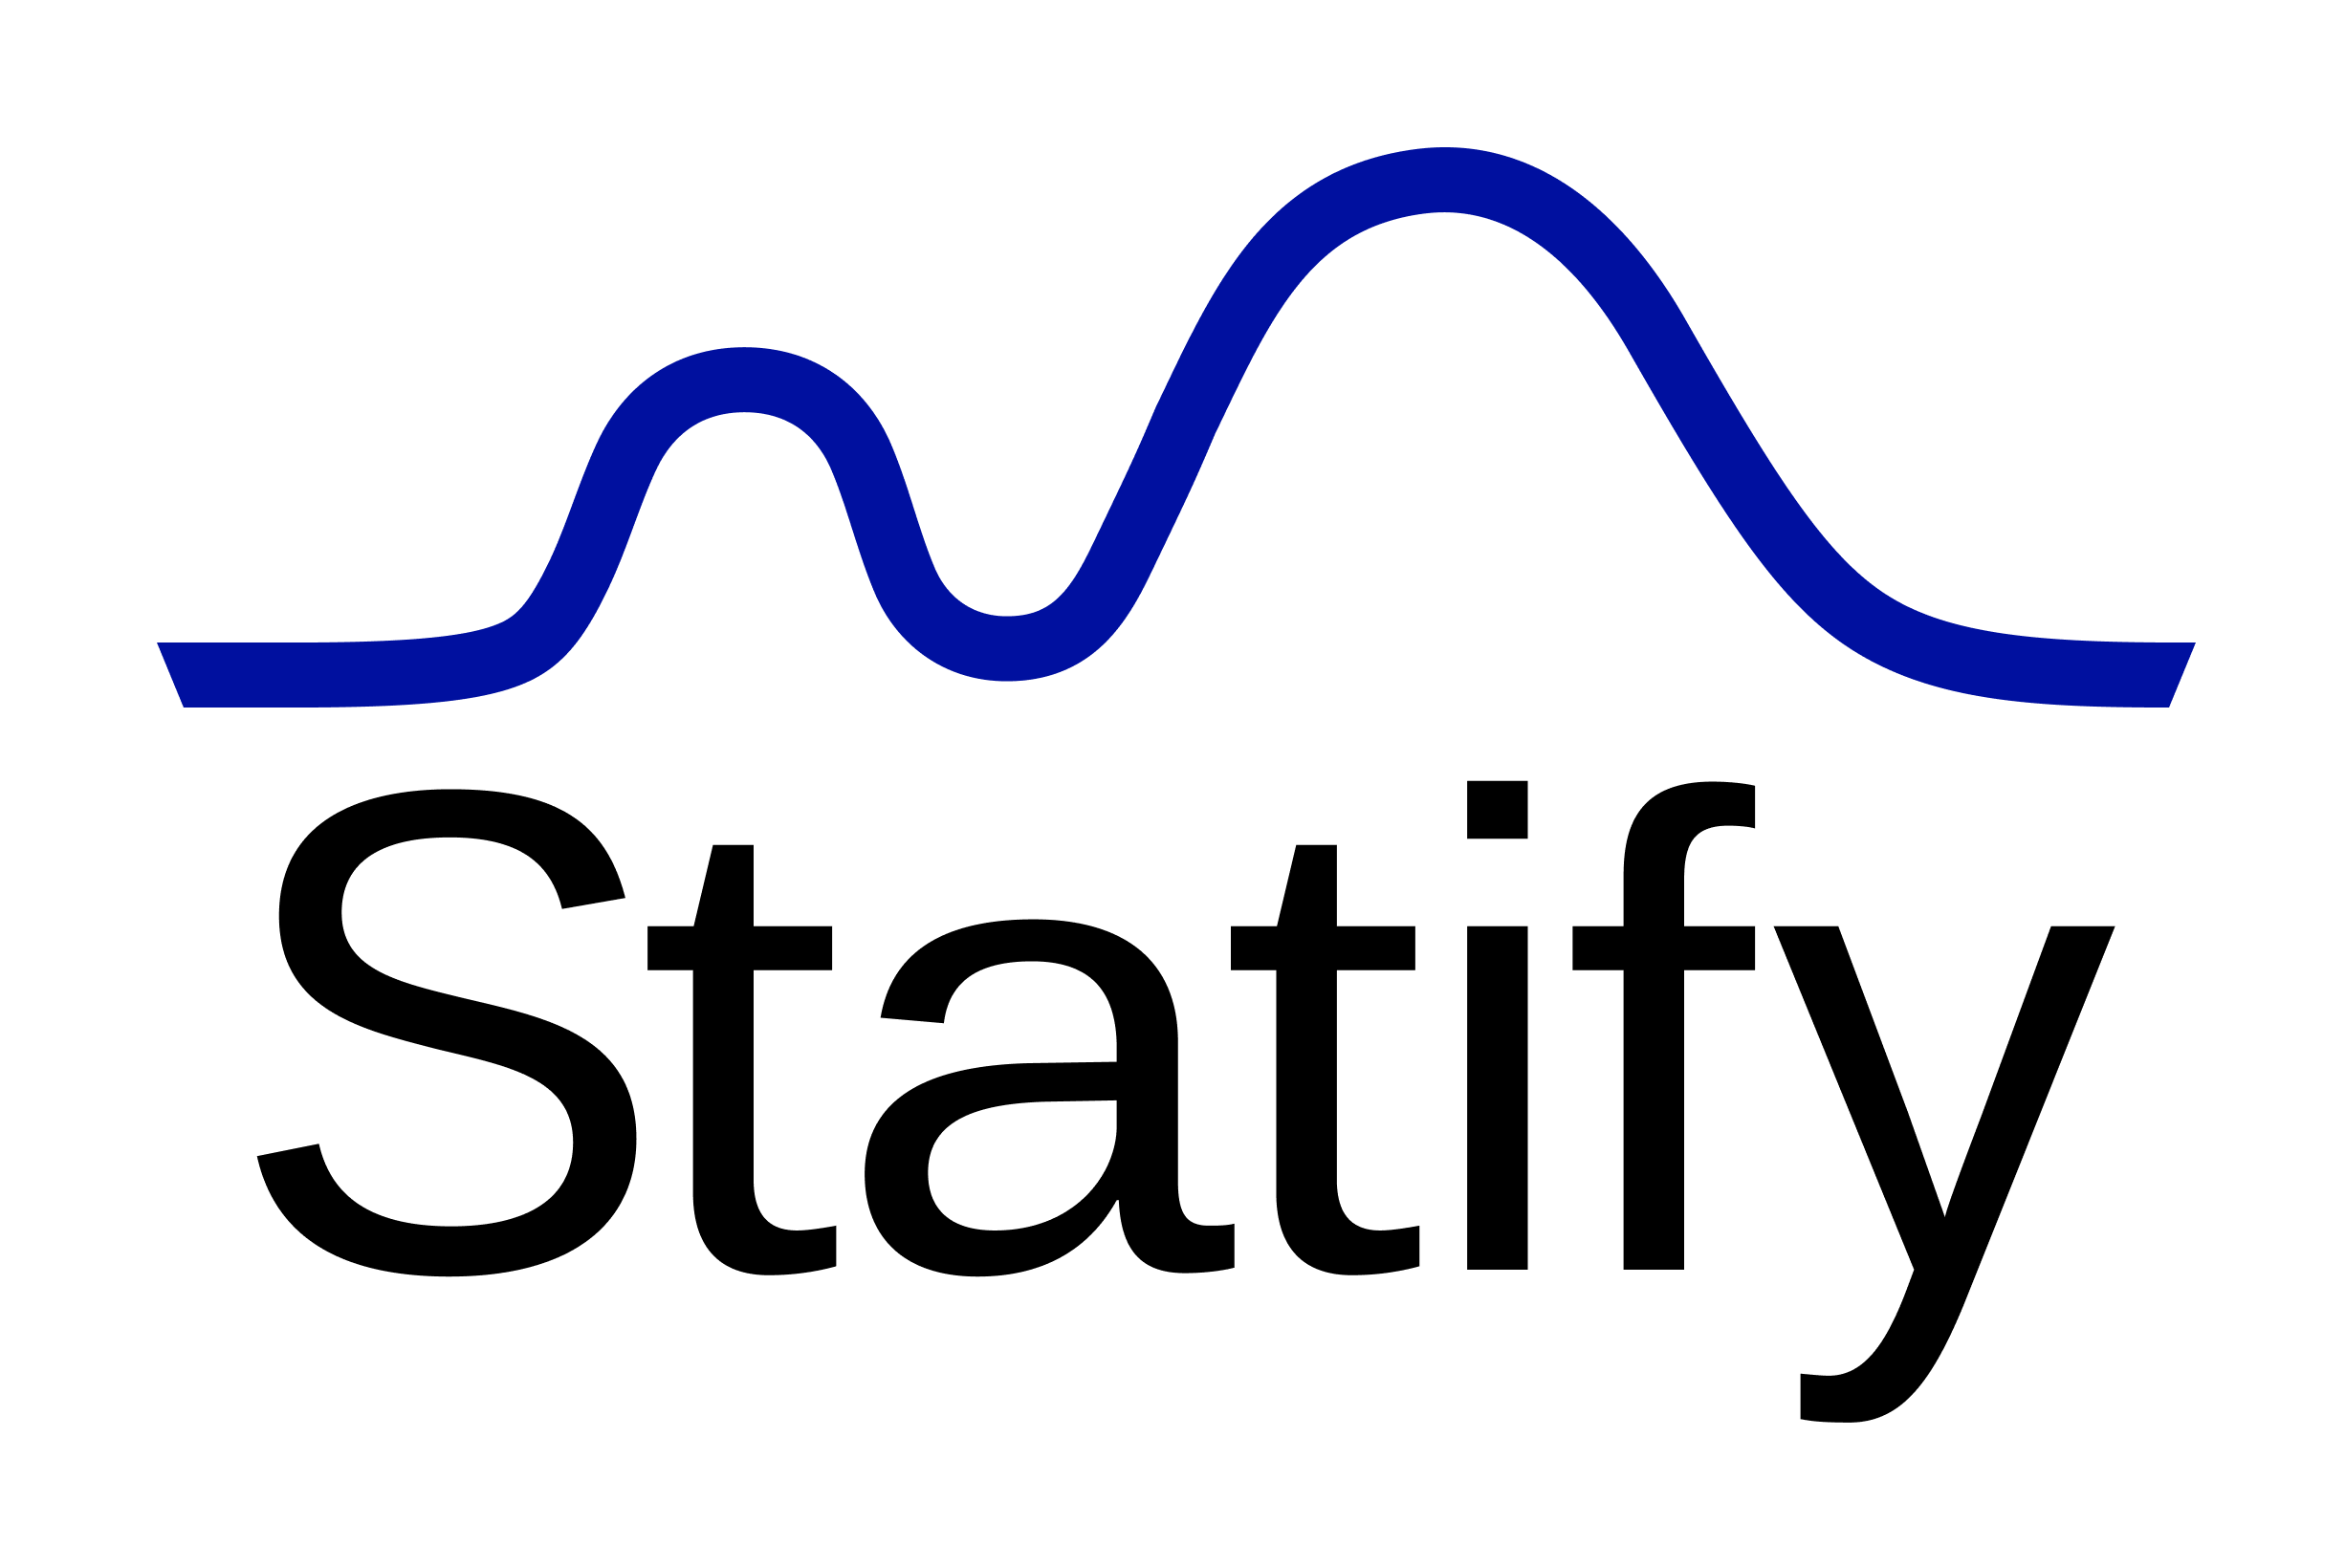
\includegraphics[width=0.3\textwidth]{figures_julyan/logo/statify.png}
}
\date{}



\definecolor{forestgreen}{rgb}{0.13, 0.55, 0.13}
\definecolor{darkblue}{rgb}{0.0, 0.0, 0.65}
\definecolor{violet2}{rgb}{0.5,0,0.5}
\definecolor{orange2}{rgb}{0.8, 0.1, 0.1}       
\definecolor{red2}{rgb}{1, 0.4, 0}






% specifics Julyan
\setlength{\parskip}{0.5\baselineskip}%
\setlength{\parindent}{0pt}%
% end specifics Julyan


\newcommand{\T}{{\text{\tiny\sffamily\upshape\mdseries T}}}
\newcommand{\bx}{\boldsymbol{x}}
\newcommand{\bmu}{\boldsymbol{\mu}}
\newcommand{\bh}{\boldsymbol{h}}
\newcommand{\bb}{\boldsymbol{b}}
\newcommand{\bV}{\boldsymbol{V}}
\newcommand{\bW}{\boldsymbol{W}}
%\newcommand{\bU}{\boldsymbol{U}}
\newcommand{\bH}{\boldsymbol{H}}
\newcommand{\bw}{\boldsymbol{w}}
\newcommand{\bz}{\boldsymbol{z}} 
\newcommand{\bX}{\boldsymbol{X}} 
\newcommand{\by}{\boldsymbol{y}} 
\newcommand{\bg}{\boldsymbol{g}} 
\newcommand{\bv}{\boldsymbol{v}} 
\newcommand{\be}{\boldsymbol{e}} 
\newcommand{\boldf}{\boldsymbol{f}} 
\newcommand{\Lnorm}{\mathcal{L}} 
\newcommand{\R}{\mathbb{L}} 
\newcommand{\subW}{subW} % \normalfont 

\def\simiid{\overset{\text{iid}}{\sim}}
\def\simind{\overset{\text{ind}}{\sim}}
%\newcommand{\ind}{\perp\!\!\!\!\perp} 

% for BNP part

%% Michal's

\newcommand{\PrecisionParam}{\alpha}
\newcommand{\Dir}{\text{Dir}}
\newcommand{\Beta}{\text{Beta}}

\usepackage{mathtools}

\newcommand\diseq{\stackrel{\mathclap{\normalfont\mbox{\small{d}}}}{=}}


%\newcommand{\distas}[1]{\mathbin{\overset{#1}{\kern\z@\sim}}}%
\newsavebox{\mybox}\newsavebox{\mysim}
\newcommand{\distras}[1]{%
  \savebox{\mybox}{\hbox{\kern3pt$\scriptstyle#1$\kern3pt}}%
  \savebox{\mysim}{\hbox{$\sim$}}%
  \mathbin{\overset{#1}{\kern\z@\resizebox{\wd\mybox}{\ht\mysim}{$\sim$}}}%
}


%% mathbb
\newcommand{\bbC}{\mathbb{C}}
\newcommand{\indic}{\mathds{1}}
\newcommand{\F}{\mathbb{F}}
\newcommand{\X}{\mathbb{X}}
%\newcommand{\Z}{\mathbb{Z}}
\newcommand{\Sd}{\mathbb{S}}
\newcommand{\Y}{\mathbb{Y}}


%% mathds
%\newcommand{\R}{\mathbb{R}}
\newcommand{\E}{\mathrm{E}}
\newcommand{\Cov}{\mathsf{Cov}}
\newcommand{\Var}{\mathsf{Var}}
\newcommand{\N}{\mathds{N}}
\newcommand{\Nbb}{\mathds{N}}
\renewcommand{\P}{\mathds{P}}

\newcommand{\Xn}{X^n}



%%% Script letters
\newcommand{\Bcr}{\mathscr{B}}
\newcommand{\Fcr}{\mathscr{F}}
\newcommand{\Dcr}{\mathscr{D}}
\newcommand{\Icr}{\mathscr{I}}
\newcommand{\Lcr}{\mathscr{L}}
\newcommand{\Pcr}{\mathscr{P}}
\newcommand{\Xcr}{\mathscr{X}}
\newcommand{\Mcr}{\mathscr{M}}
\newcommand{\Ycr}{\mathscr{Y}}
\newcommand{\Acr}{\mathscr{A}}
\newcommand{\Gcr}{\mathscr{G}}
\newcommand{\Vcr}{\mathscr{V}}

%%% Mathfrak
\newcommand{\Xf}{\mathfrak{X}}
\newcommand{\Sf}{\mathfrak{\sigma}}

\newcommand{\ddr}{\mathrm{d}}
\newcommand{\edr}{\mathrm{e}}
\newcommand{\idr}{\mathrm{i}}

%\renewcommand{\abstractname}{SUMMARY}
\renewcommand{\theparagraph}{\arabic{paragraph}}
%\numberwithin{equation}{paragraph}

\newcommand{\Rt}{\Rightarrow}
\newcommand{\rt}{\rightarrow}
\newcommand{\lrt}{\longrightarrow}
\newcommand{\Lerit}{\Leftrightarrow}
\newcommand{\dimo}{\underline{\textsc{Proof.}} }
\newcommand{\cc}{\hfill $\square$}
\newcommand{\ind}{\bm 1}
\newcommand{\bm}{\mathbf}
\newcommand{\var}{\varepsilon}
\newcommand{\intre}{\int_{\mathbb{R}}}
\newcommand{\intoinf}{\int_0^{+\infty}}

\newcommand{\Bc}{\mathcal{B}}
\newcommand{\Cc}{\mathcal{C}}
\newcommand{\Fc}{\mathcal{F}}
\newcommand{\Lc}{\mathcal{L}}
\newcommand{\Nc}{\mathcal{N}}
\newcommand{\Pc}{\mathcal{P}}
\newcommand{\Ic}{\mathcal{I}}
\newcommand{\Zc}{\mathcal{Z}}

\newcommand{\dir}{P_{\alpha}}
\newcommand{\ep}{\varepsilon}
\newcommand{\e}{\mathsf{E}}
\newcommand{\trunc}{{\sigma,\tau}}
%\newcommand{\p}{\mathbb{P}}
\newcommand{\prob}{\mathsf{P}}
\newcommand{\Ga}{\Gamma_\alpha}
\newcommand{\Ma}{M_\alpha}
\newcommand{\Ua}{U_\alpha}
\newcommand{\Va}{V_\alpha}
\newcommand{\wt}{\widetilde}

\def\simind{\stackrel{\mbox{\scriptsize{ind}}}{\sim}}
\def\simiid{\stackrel{\mbox{\scriptsize{iid}}}{\sim}}

% altro
\newcommand{\mt}{{\mu}} % misura completamente aleatoria (CRM)
\newcommand{\hti}{{h}}
\newcommand{\St}{{S}}
\newcommand{\pt}{\tilde{p}} % legge aleatoria
\newcommand{\At}{\tilde{A}} %
\newcommand{\Bt}{\tilde{B}} %
\newcommand{\Lz}{\mathcal{L}_Z} % legge di Z

\newcommand{\AC}{\\[7pt]} % a capo
\newcommand{\La}{\mathcal{L}}
%\newcommand{\p}{\mathbb{P}}
%\newcommand{\AC}{\\[7pt]}
\newcommand{\bn}{\bar{n}}
\newcommand{\I}{\mathcal{I}}
\newcommand{\C}{\mathcal{C}}
\newcommand{\Ac}{\mathcal{A}}

% Ju
\newcommand{\vertju}{\,\vert\,}
\newcommand{\twoPD}{two-parameter Poisson-Dirichlet process\xspace}
\newcommand{\DP}{\text{Dirichlet process}\xspace}
\newcommand{\levy}{L\'evy\xspace}
\newcommand{\Gumbel}{\text{Gumbel}\xspace}
\newcommand{\Exp}{\text{Exp}\xspace}
\def\simiid{\stackrel{\mbox{\scriptsize{iid}}}{\sim}}
\def\simind{\stackrel{\mbox{\scriptsize{ind}}}{\sim}}
\def\proptoind{\stackrel{\mbox{\scriptsize{ind}}}{\propto}}
\newcommand{\citp}[1]{\textcolor{blue}{\citep{#1}}}
\newcommand{\citt}[1]{\textcolor{blue}{\citet{#1}}}


\newcommand{\crms}{completely random measures\xspace}
\newcommand{\crm}{completely random measure\xspace}
\newcommand{\CRM}{CRM\xspace}
\newcommand{\Crms}{Completely random measures\xspace}
\newcommand{\Crm}{Completely random measure\xspace}
\newcommand{\muA}{\tilde \mu(A)\xspace}
\newcommand{\muX}{\tilde \mu(\X)\xspace}
\newcommand{\cnkpar}{\binom{n}{k_1\cdots k_n}}
\newcommand{\cnkfact}{\frac{n!}{k_1!\ldots k_n!}}
\newcommand{\g}{\mathbf{g}}
\newcommand{\FK}{\citeauthor{ferguson1972representation}\xspace} 
\newcommand{\FKa}{\citeauthor{ferguson1972representation} algorithm\xspace} 
\newcommand{\BP}{\ensuremath{\text{BP}}\xspace} 
\newcommand{\BeP}{\ensuremath{\text{BeP}}\xspace} 
%\newcommand{\gg}{\ensuremath{\text{GG}}\xspace} 
\newcommand{\GG}{generalized gamma process\xspace} 
\newcommand{\SBP}{stable-beta process\xspace} 
\newcommand{\IBP}{Indian buffet process\xspace} 
\newcommand{\IG}{inverse-Gaussian process\xspace} 
\newcommand{\NMC}{N_{\text{\tiny{FK}}}} 
\newcommand{\EFK}{\mathbb{E}_{\text{\tiny{FK}}}}


\def\unit{\mathbf{1}}
\def\bc{c}
\def\prob{\mathbb{P}}
\def\bc{c}
\def\Ac{\mathcal{A}}
\def\VI{\text{VI}}
\def\En{\text{H}}
\def\B{\text{B}}
%\def\argmax{\text{argmax}}
\DeclareMathOperator*{\argmax}{arg\,max}
\DeclareMathOperator*{\argmin}{arg\,min}
\def\1{\unit}


%% notation
\DeclareMathOperator*{\argmax}{arg\,max}
\DeclareMathOperator*{\argmin}{arg\,min}
\newcommand{\cA}{\mathcal{A}}
\newcommand{\cS}{\mathcal{S}}
\newcommand{\cF}{\mathcal{F}}
\newcommand{\cX}{\mathcal{X}}
\newcommand{\cY}{\mathcal{Y}}
\newcommand{\cZ}{\mathcal{Z}}
\newcommand{\cN}{\mathcal{N}}
\newcommand{\cO}{\mathcal{O}}
\renewcommand{\leq}{\leqslant}
\renewcommand{\geq}{\geqslant}
\renewcommand{\phi}{\varphi}
\renewcommand{\epsilon}{\varepsilon}
\renewcommand{\d}{ {\rm d}}
\renewcommand{\emptyset}{\varnothing}


\usepackage{tikz}


\begin{document}
\begin{frame}
\maketitle
\end{frame}


\begin{frame}{Outline}
	\tableofcontents[pausesections,subsectionstyle=hide,subsubsectionstyle=hide]
\end{frame}


%%%%%%%%%%%%%%%%%%%%%%
\section{Introduction}
%%%%%%%%%%%%%%%%%%%%%%

\begin{frame}{What comes to \emph{your} mind when you hear ``Bayesian deep learning''?}
\end{frame}

%\begin{frame}{Deep neural networks}
%\begin{center}
%	\includegraphics[width=\textwidth]{figures_julyan/bnn}
%\end{center}
%\end{frame}


\begin{frame}{Deep neural networks Achilles heels}
\begin{center}
\only<1>{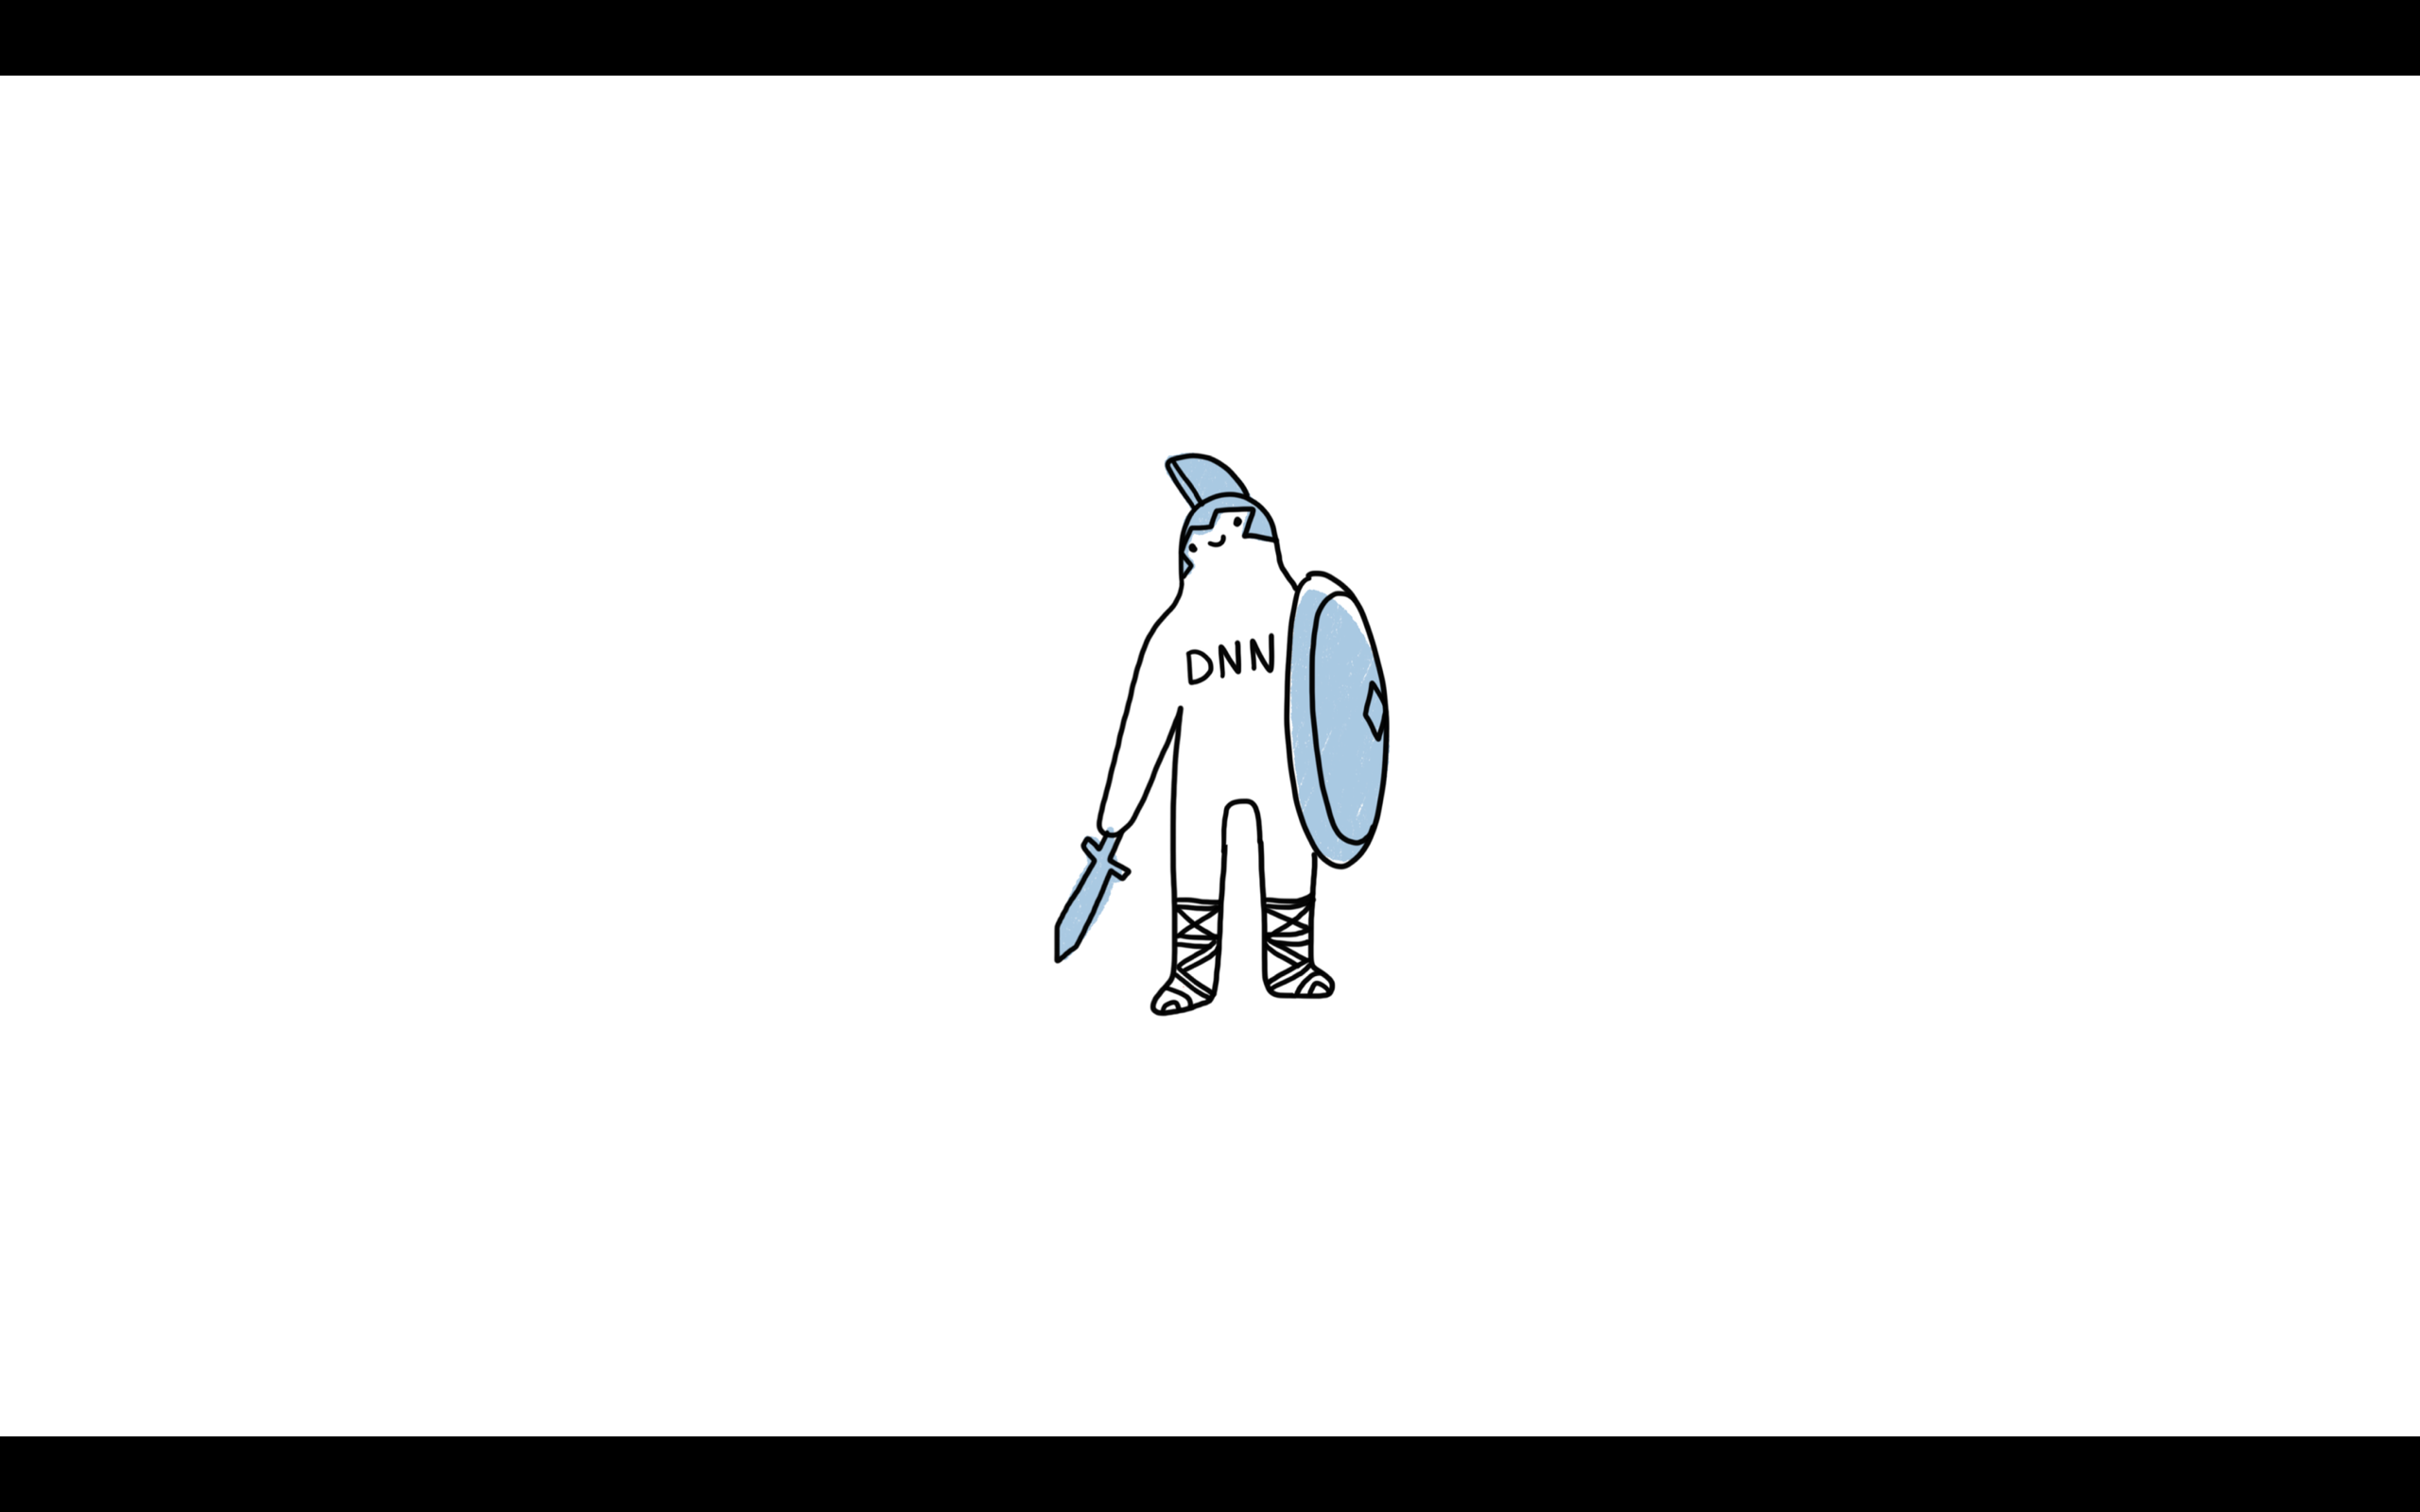
\includegraphics[height=.8\textheight,trim={12cm 6cm 12cm 8cm},clip]{figures_julyan/bdl/achilles1}}
\only<2>{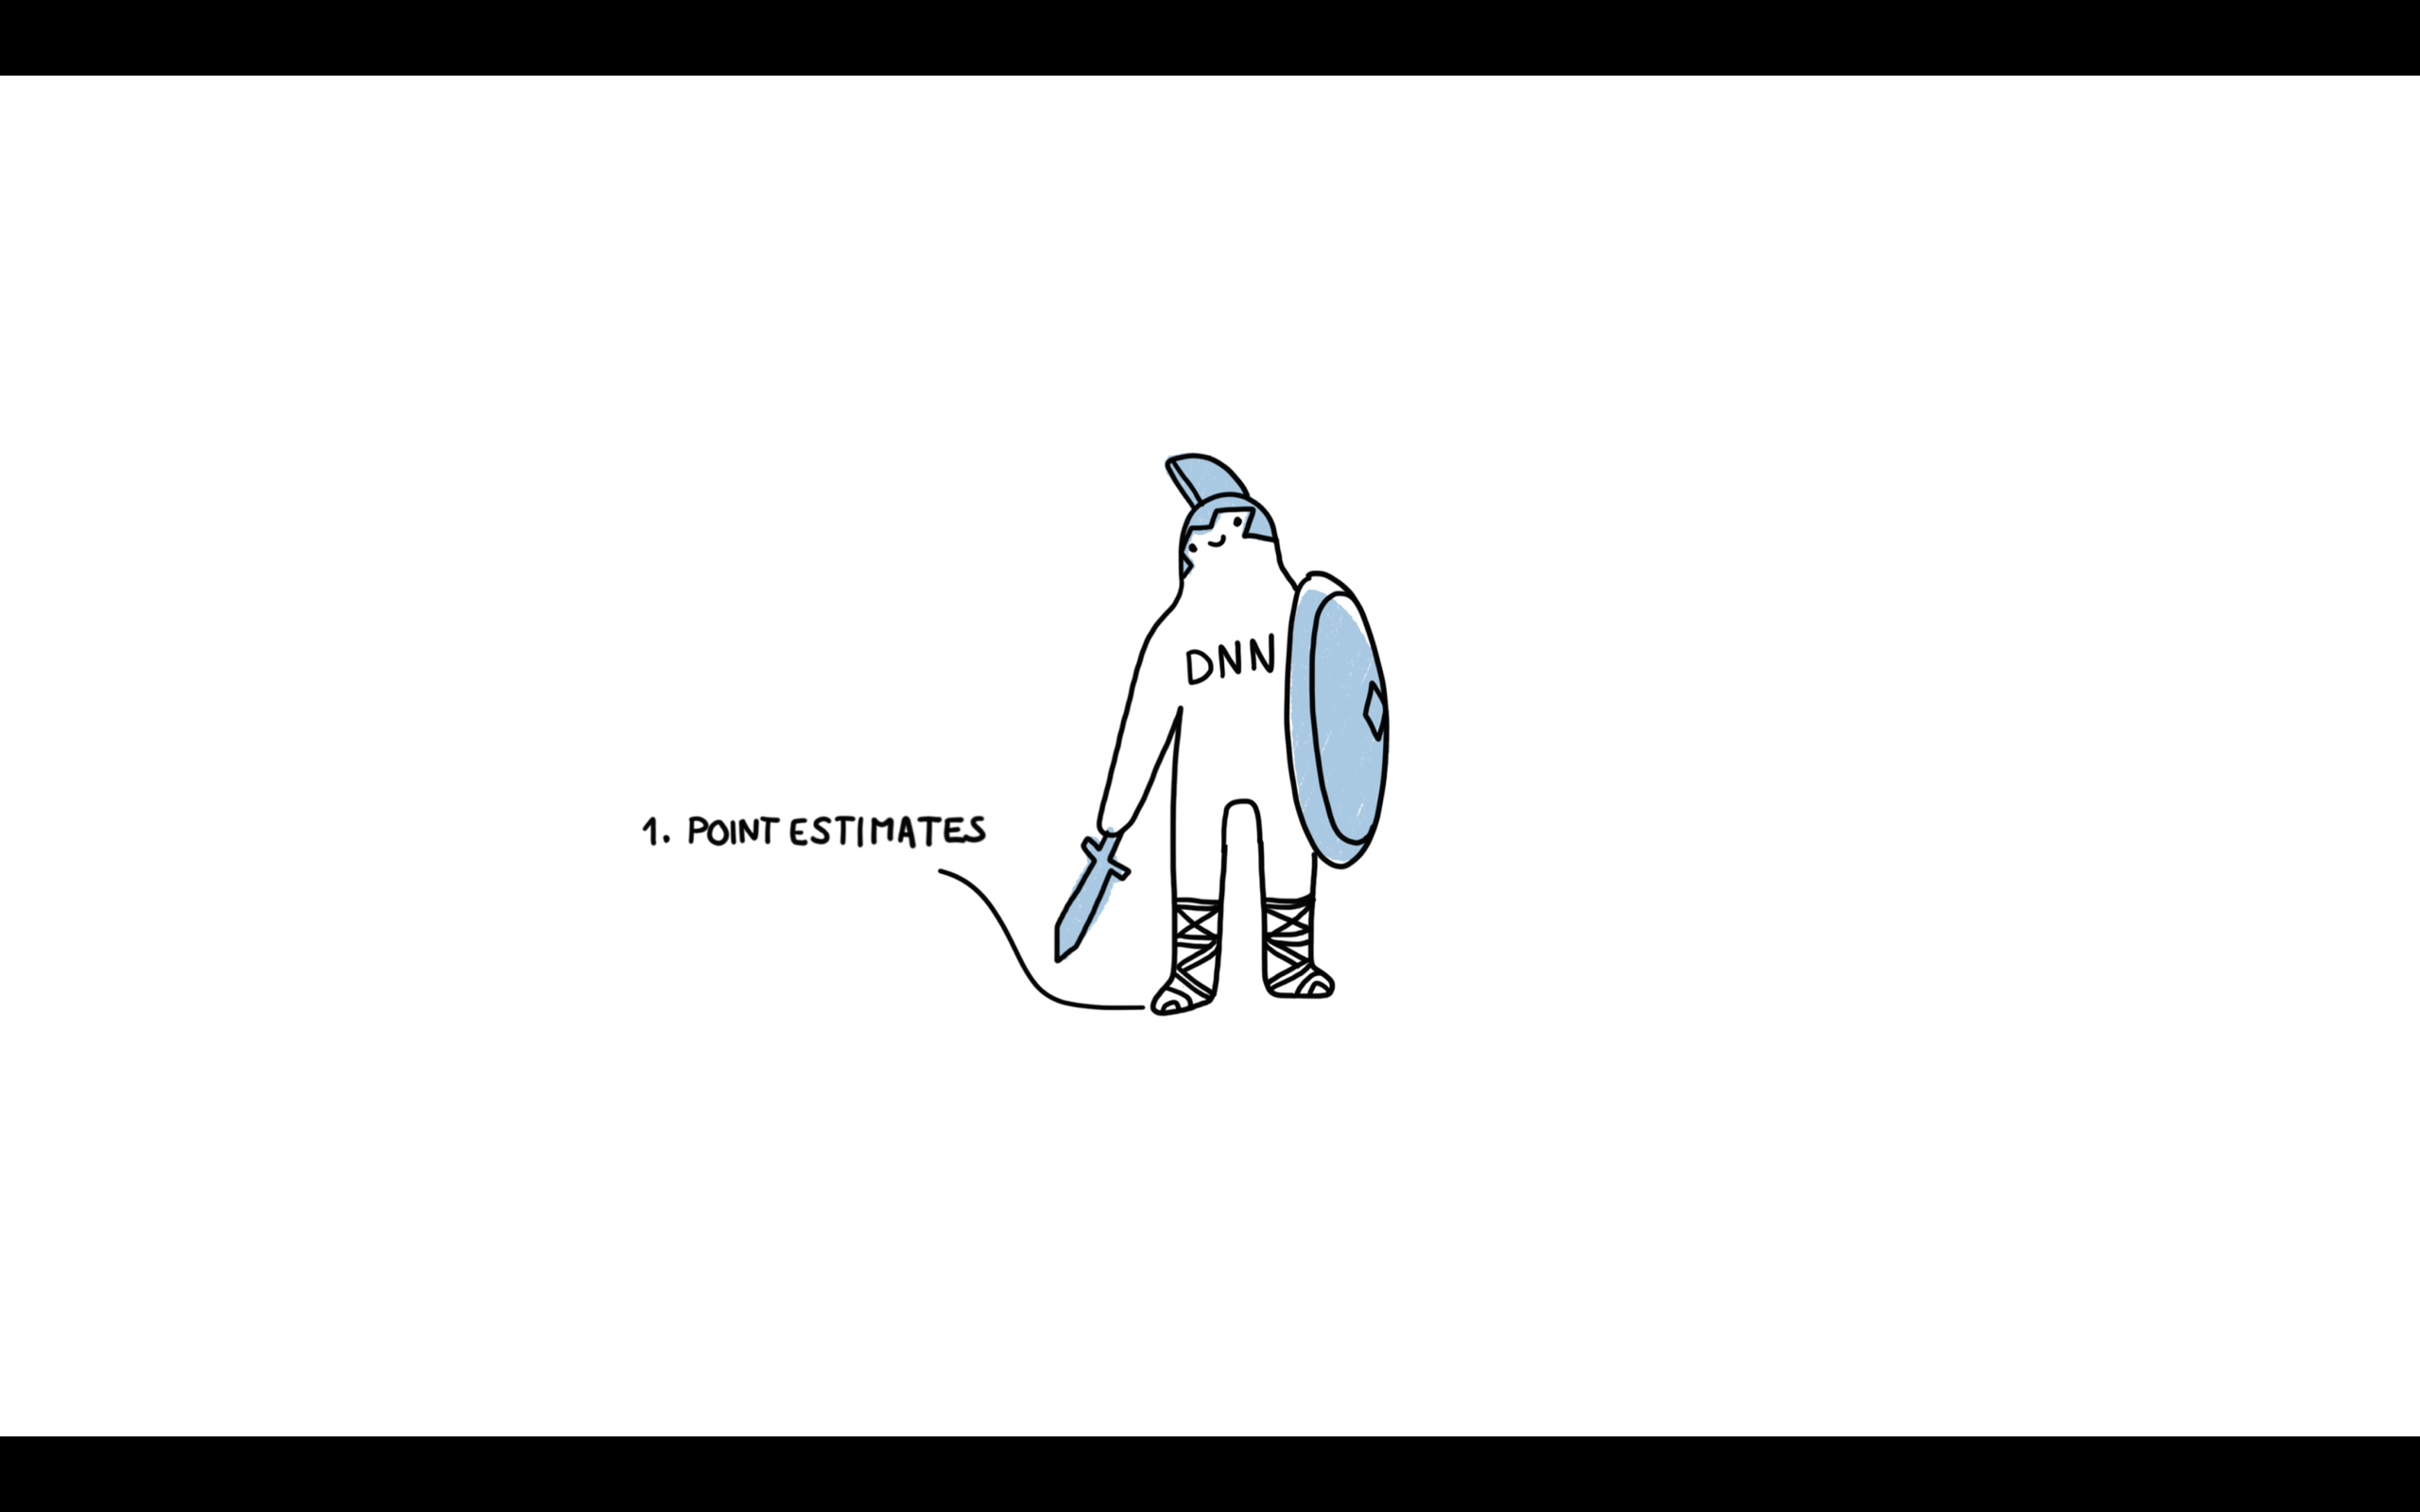
\includegraphics[height=.8\textheight,trim={12cm 6cm 12cm 8cm},clip]{figures_julyan/bdl/achilles2}}
\only<3>{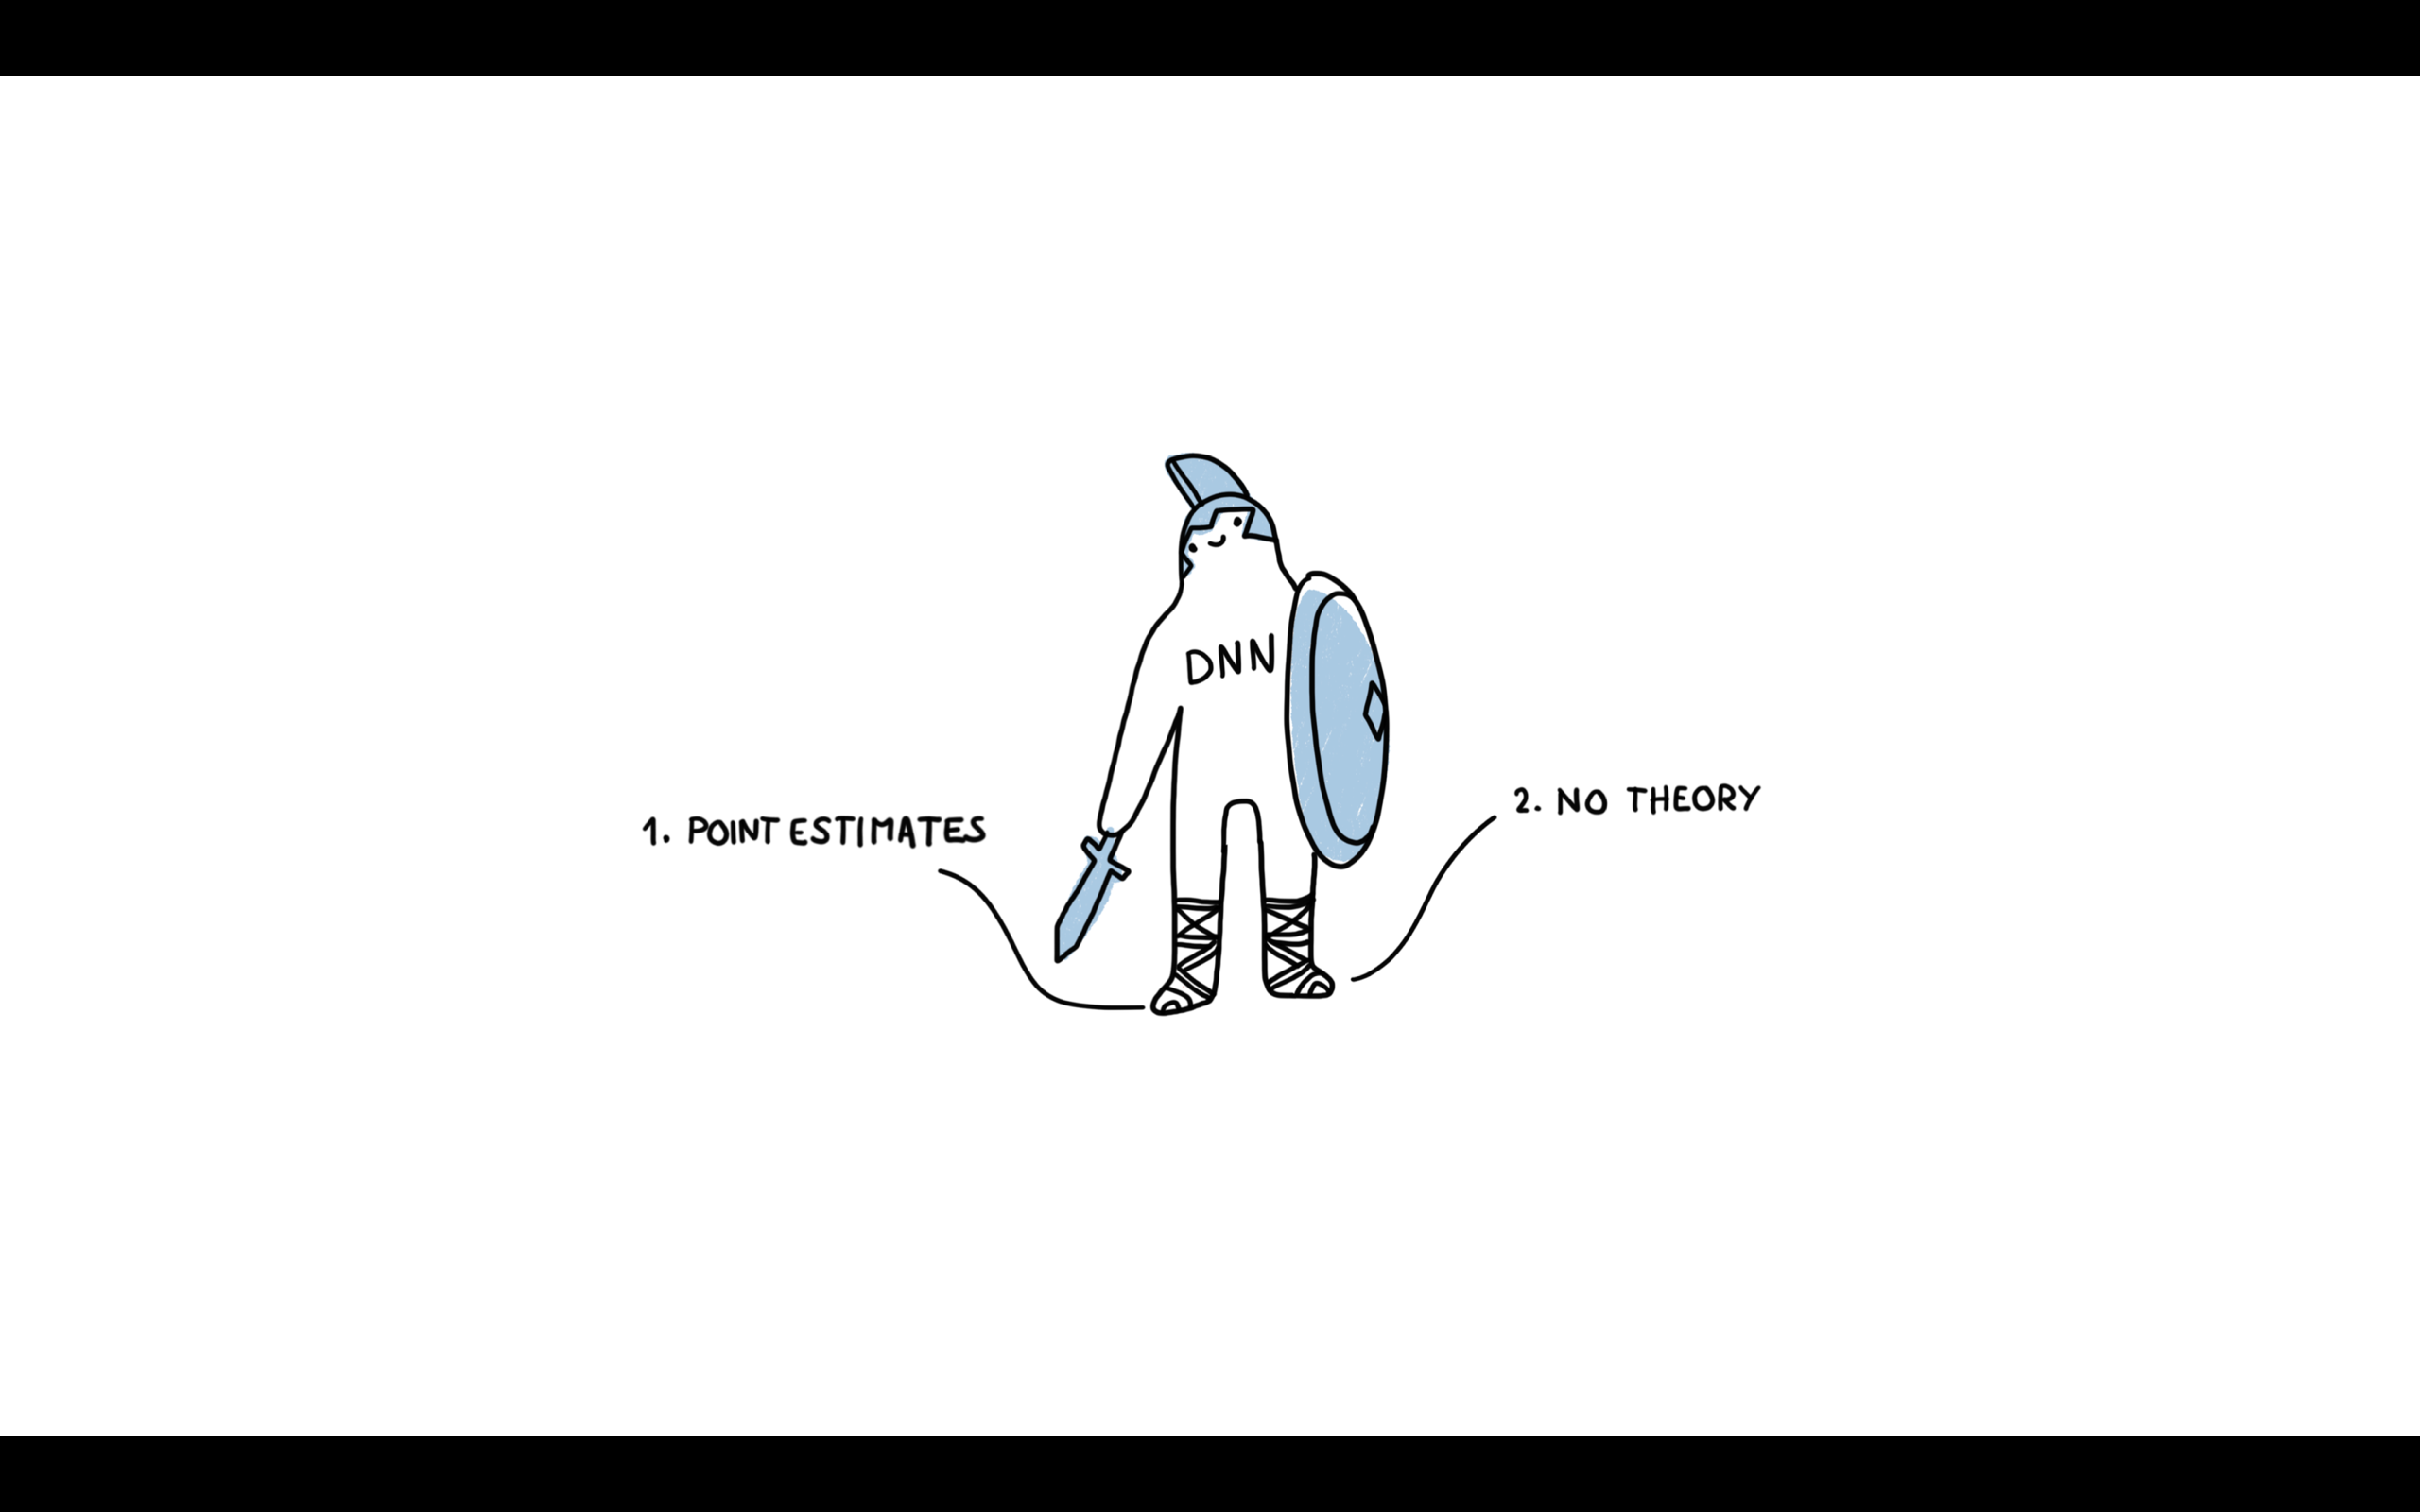
\includegraphics[height=.8\textheight,trim={12cm 6cm 12cm 8cm},clip]{figures_julyan/bdl/achilles3}}
\end{center}
\end{frame}

\begin{frame}{Different flavours of neural networks \citep{jospin2020handson}}
\begin{center}
\begin{tabular}{cc}
	\visible<1->{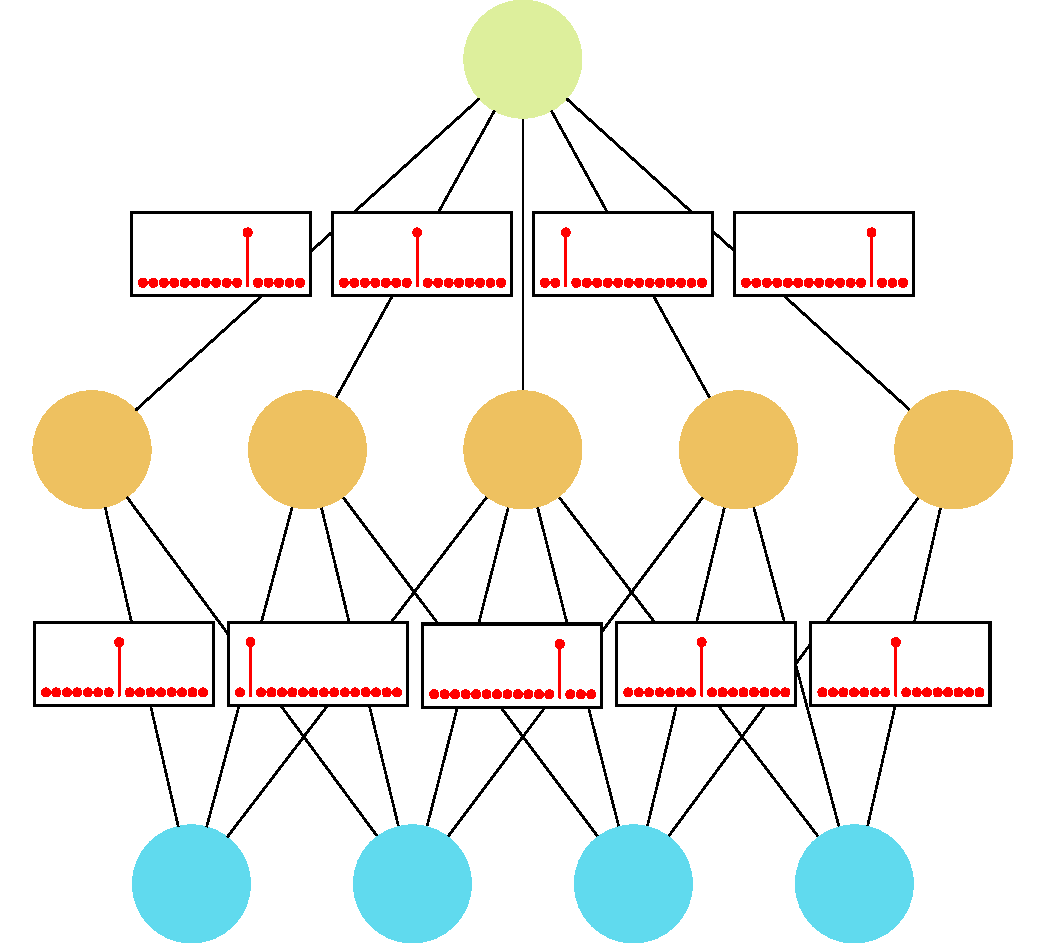
\includegraphics[width=.3\textwidth]{figures_julyan/bdl/hands-on/schemaNNPE}} &
	\visible<2->{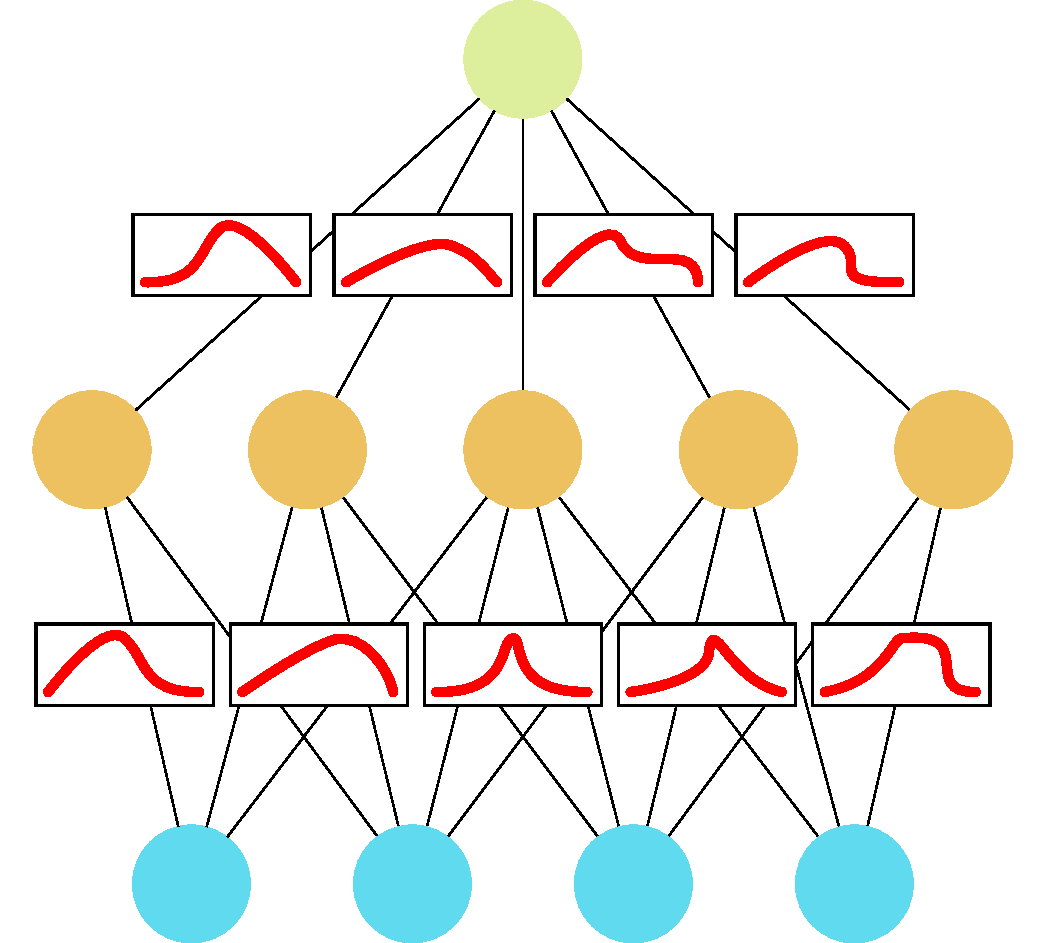
\includegraphics[width=.3\textwidth]{figures_julyan/bdl/hands-on/schemaNNStochastic}}\\
	\visible<1->{Point estimate NN} & 
	\visible<2->{BNN w/ random weights}\\
	\visible<3->{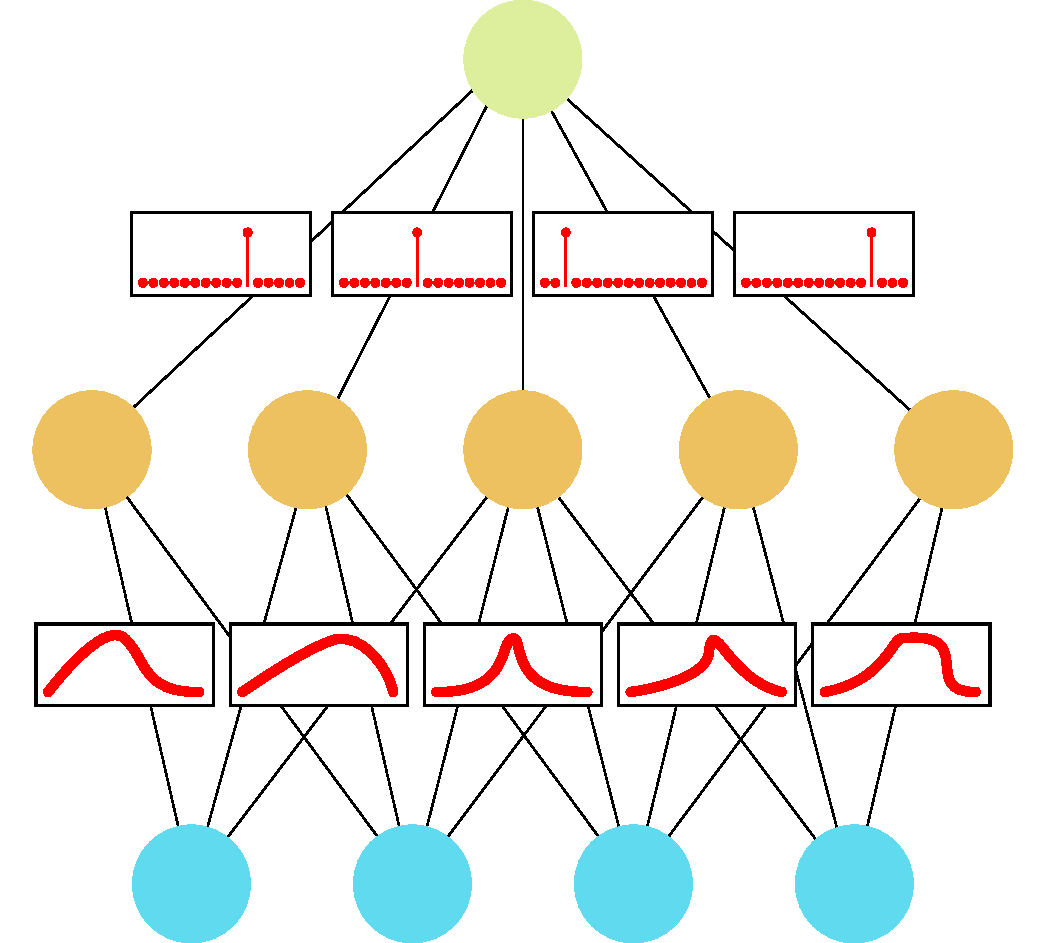
\includegraphics[width=.3\textwidth]{figures_julyan/bdl/hands-on/schemaNNLastLayer}} &
	\visible<4->{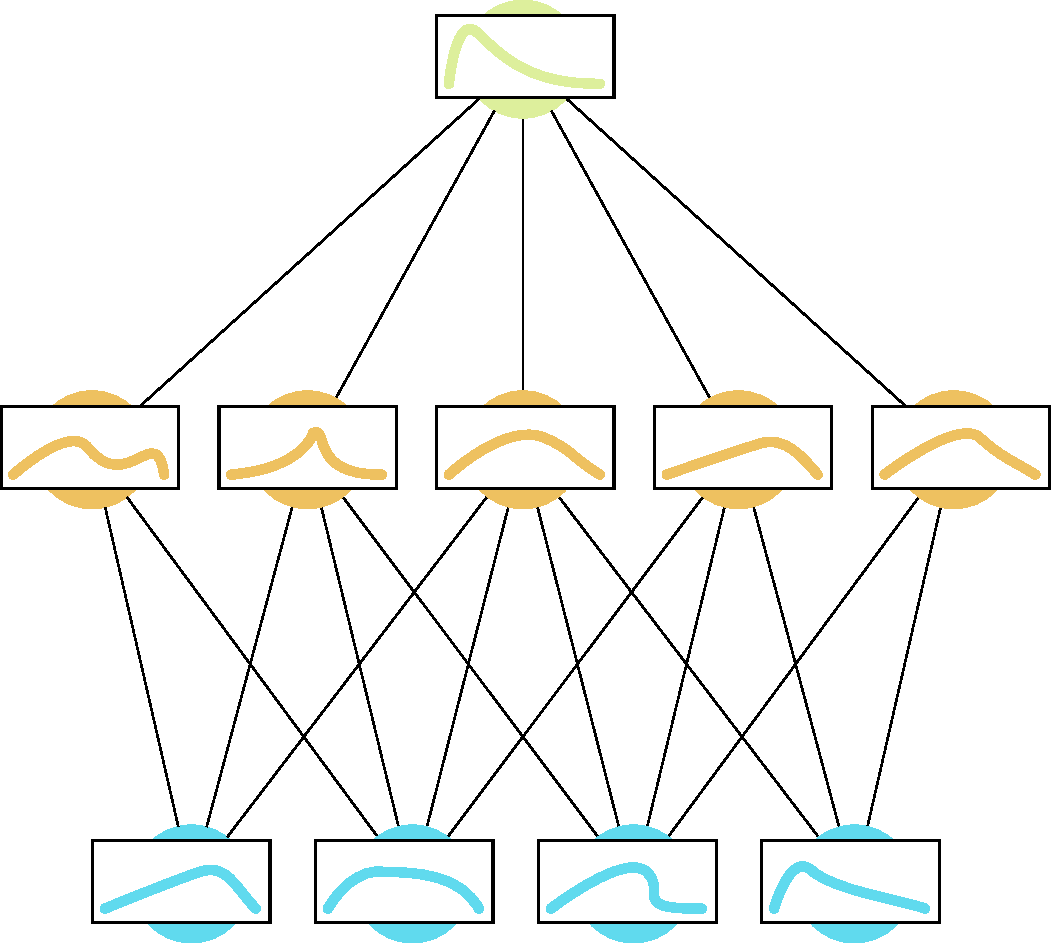
\includegraphics[width=.3\textwidth]{figures_julyan/bdl/hands-on/schemaNNTransfert}}\\
	\visible<3->{BNN w/ last-layer rd weights} & 
	\visible<4->{BNN w/ random activations}
\end{tabular}
\end{center}
\end{frame}


\begin{frame}{Useful references}
\begin{itemize}
	\item \alert{First substantial reference}: Chapter 17 on BNNs by \fullcite{murphy2023probabilisticMLadvanced}
	\item  \alert{Review papers}: \citet{jospin2020hands,abdar2021review,goan2020bayesian,fortuin2021priors,ashukha2020pitfalls,band2021benchmarking,nado2021uncertainty}
	\item \alert{Our review paper}: \fullcite{arbel2023primer}
\end{itemize}
\end{frame}
	

%\begin{frame}{Bayesian neural networks}
%\begin{center}
%	\only<1>{%\hskip-3cm%\vspace{-2cm}
%	\includegraphics[width=1.1\textwidth]{figures_julyan/bnn1}}
%	\only<2>{\includegraphics[width=1.1\textwidth]{figures_julyan/bnn2}}
%	\only<3>{\includegraphics[width=1.1\textwidth]{figures_julyan/bnn3}}
%\end{center}
%\end{frame}




%%%%%%%%%%%%%%%%%%%%%%%%%%%%%%%%%%%%%%%%%%%%%%%%%%%%%%%%
\section{Feed-forward neural networks}
%%%%%%%%%%%%%%%%%%%%%%%%%%%%%%%%%%%%%%%%%%%%%%%%%%%%%%%%

\begin{frame}{Neural networks notations}

\begin{figure}[ht!]
\begin{center}
\scalebox{.8}{
\tikzset{%
  input/.style={
      circle,
      draw,
      color={rgb, 255:red, 107; green, 65; blue, 144 },
      draw opacity=1,
      fill={rgb, 255:red, 107; green, 65; blue, 144 },
      fill opacity=0.48,
      minimum size=0.5cm
    },
    every neuron/.style={
      circle,
      draw,
      color={rgb, 255:red, 65; green, 117; blue, 5 },
      draw opacity=1,
      fill={rgb, 255:red, 65; green, 117; blue, 5 },
      fill opacity=0.48,
      minimum size=0.5cm
    },
    neuron missing/.style={
      draw=none, 
      fill=none,
      scale=1,
      text height=0.333cm,
      execute at begin node=\color{black}$\vdots$
    },
    output/.style={
      circle,
      draw,
      color={rgb, 255:red, 107; green, 65; blue, 144 },
      draw opacity=1,
      fill={rgb, 255:red, 107; green, 65; blue, 144 },
      fill opacity=0.48,
      minimum size=0.5cm
    },
}
\begin{tikzpicture}[x=1.2cm, y=0.8cm, >=stealth]

\foreach \m/\l [count=\y] in {1,2,3,missing,4}
  \node [input/.try, neuron \m/.try] (input-\m) at (0,2.2-\y) {};

\foreach \m [count=\y] in {1,2,missing,3}
  \node [every neuron/.try, neuron \m/.try ] (firsthidden-\m) at (2,1.9-\y*1.1) {};

\foreach \m [count=\y] in {1,2,missing,3}
  \node [every neuron/.try, neuron \m/.try ] (secondhidden-\m) at (4,1.9-\y*1.1) {};

\foreach \m [count=\y] in {1,2,3,4}
  \node [neuron missing/.try, neuron \m/.try ] (thirdhidden-\m) at (6,1.9-\y*1.1) {};

\foreach \m [count=\y] in {1,2,missing,3}
  \node [every neuron/.try, neuron \m/.try ] 
(lasthidden-\m) at (8,1.9-\y*1.1) {};

\foreach \m [count=\y] in {1,missing,2}
  \node [output/.try, neuron \m/.try ] 
(output-\m) at (10,1.6-\y*1.1) {};



\foreach \l [count=\i] in {1,2,3,n}
  \draw [<-] (input-\i) -- ++(-1,0);
  \node [above] at (input-1.north) {$\bx$};

\foreach \l [count=\i] in {1};
\node [above] at (firsthidden-1.north) {$\bh^{(1)}$};

% \foreach \l [count=\i] in {1,2,n}
%   \node [above] at (secondhidden-\i.north) {$h^{(2)}_\l$};

\foreach \l [count=\i] in {1};
  \node [above] at (secondhidden-1.north) {$\bh^{(2)}$};

\foreach \l [count=\i] in {1}
  \node [above] at (thirdhidden-1.north) {$\bh^{(\ell)}$};

\foreach \l [count=\i] in {1,2,n}
%   \draw [->] (lasthidden-\i) -- ++(1,0);
 \node [above] at (lasthidden-1.north) {$\bh^{(L)}$};

\foreach \l [count=\i] in {1}
  \node [above] at (output-1.north) {$\by$};



\foreach \i in {1,...,4}
  \foreach \j in {1,...,3}
    \draw [->] (input-\i) -- (firsthidden-\j);

\foreach \i in {1,...,3}
  \foreach \j in {1,...,3}
    \draw [->] (firsthidden-\i) -- (secondhidden-\j);

\foreach \i in {1,...,3}
  \foreach \j in {1,...,4}
    \draw [->] (secondhidden-\i) -- (thirdhidden-\j);

\foreach \i in {1,...,4}
  \foreach \j in {1,...,3}
    \draw [->] (thirdhidden-\i) -- (lasthidden-\j);

\foreach \i in {1,...,3}
  \foreach \j in {1,...,2}
    \draw [->] (lasthidden-\i) -- (output-\j);


\foreach \l [count=\x from 0] in {\footnotesize{input}, \footnotesize{$1^{\text{st}}$ hidden}, \footnotesize{$2^{\text{nd}}$ hidden}, , \footnotesize{last hidden}, \footnotesize{output}}
  \node [align=center, above] at (\x*2,2) {\l};


\end{tikzpicture}
}
\end{center}
%\caption{Neural network architecture.}
\label{figure:nn_visualization_intro}
\end{figure}

\begin{itemize}
	\item \alert{pre-nonlinearity} $\bg^{(\ell)}=\bg^{(\ell)}(\bx)$, \alert{post-nonlinearity}  $\bh^{(\ell)}=\bh^{(\ell)}(\bx)$
\begin{align*}\label{eq:propagation}
      \bg^{(\ell)}(\bx) = \bW^{(\ell)} \bh^{(\ell - 1)} (\bx), \quad \bh^{(\ell)} (\bx) = \phi(\bg^{(\ell)}(\bx))
\end{align*}
	\item \alert{nonlinearity} or \alert{activation function}  $\phi: \mathbb{R} \to \mathbb{R}$.
	\item \alert{weight matrix} $\bW^{(\ell)}$ of dimension $H_\ell\times H_{\ell-1}$ including a bias vector
\end{itemize}

\end{frame}


\begin{frame}{Training}
Optimization problem: minimize the loss function
\begin{equation*}
    \hat \bw = \argmin_{\bw} \mathcal{L}(\bw).
\end{equation*}
With gradient-based optimization: 
\begin{equation*}
    \bw \leftarrow \bw - \eta\, \partial_{\bw} \mathcal{L}(\bw).
\end{equation*}
$\eta > 0$ is a \alert{step size}, or \alert{learning rate}. Gradients are computed as products of gradients between each layer \alert{from right to left}, a procedure called \alert{backpropagation}~\citep{rumelhart1986learning}.

Gradients are approximated on randomly chosen subsets called \alert{batches}: stochastic gradient descent, SGD~\citep{robbins1951stochastic}. See survey of optimization methods by\citet{sun2019survey}.
\end{frame}



\begin{frame}{Architecture choice}

\begin{itemize}
	\item \alert{Convolutional neural networks (CNN)} are widely used in computer vision.
	\item \alert{Recurrent neural networks (RNN)} are advantageous for sequential data, designed to save the output of a layer by adding it back to the input~\citep{hochreiter1997long}.
	\item \alert{Residual neural networks (ResNet)} have residual blocks which add the output from the previous layer to the layer ahead, so-called \alert{skip-connections}~\citep{he2016deep}. Allows very deep  training.
\end{itemize}
\end{frame}



\begin{frame}{Expressiveness}
Expressiveness describes neural networks’ ability to approximate functions \citep{cybenko1989approximation, funahashi1989approximate, hornik1989multilayer,barron1994approximation}. 

\begin{block}{Universal approximation theorem}
	Neural networks of one hidden layer and suitable activation function can approximate any continuous function on a compact domain, say $f: [0,1]^N \to \mathbb{R}$, to any desired accuracy.
\end{block}

\alert{But} the size of such networks may be \alert{exponential in the input dimension $N$}, which makes them highly prone to overfitting as well as impractical.

Width-depth trade-offs studied by \citet{chatziafratis2020depth,chatziafratis2020better}.

\end{frame}



\begin{frame}[allowframebreaks]{Generalization and overfitting}
\alert{Classical regime}


%\begin{figure}[ht!]
\scalebox{.85}{
\tikzset{every picture/.style={line width=0.75pt}} %set default line width to 0.75pt        

\begin{tikzpicture}[x=0.75pt,y=0.75pt,yscale=-1,xscale=1]
%uncomment if require: \path (0,300); %set diagram left start at 0, and has height of 300

%Straight Lines [id:da29796459405845743] 
\draw [color={rgb, 255:red, 0; green, 0; blue, 0 }  ,draw opacity=1 ]   (35.5,125) -- (134.5,69) ;
%Curve Lines [id:da14047940071049814] 
\draw    (402.5,125) .. controls (427,122) and (440.5,82) .. (456.5,109) .. controls (472.5,136) and (477.5,79) .. (500.5,113) ;
%Curve Lines [id:da34435969303741376] 
\draw    (227.5,120) .. controls (258.5,91) and (281.5,94) .. (318.5,105) ;
%Straight Lines [id:da8707454895547219] 
\draw [color={rgb, 255:red, 74; green, 74; blue, 74 }  ,draw opacity=1 ]   (30.5,160) -- (147.5,160) ;
%Straight Lines [id:da6627752597131152] 
\draw [color={rgb, 255:red, 74; green, 74; blue, 74 }  ,draw opacity=1 ]   (30.5,160) -- (30.5,49) ;
%Shape: Circle [id:dp44683416668789633] 
\draw  [color={rgb, 255:red, 65; green, 117; blue, 5 }  ,draw opacity=1 ][fill={rgb, 255:red, 65; green, 117; blue, 5 }  ,fill opacity=0.68 ] (49,142) .. controls (49,139.24) and (51.24,137) .. (54,137) .. controls (56.76,137) and (59,139.24) .. (59,142) .. controls (59,144.76) and (56.76,147) .. (54,147) .. controls (51.24,147) and (49,144.76) .. (49,142) -- cycle ;
%Shape: Circle [id:dp0437110253920846] 
\draw  [color={rgb, 255:red, 65; green, 117; blue, 5 }  ,draw opacity=1 ][fill={rgb, 255:red, 65; green, 117; blue, 5 }  ,fill opacity=0.68 ] (72,129) .. controls (72,126.24) and (74.24,124) .. (77,124) .. controls (79.76,124) and (82,126.24) .. (82,129) .. controls (82,131.76) and (79.76,134) .. (77,134) .. controls (74.24,134) and (72,131.76) .. (72,129) -- cycle ;
%Shape: Circle [id:dp9685072008877114] 
\draw  [color={rgb, 255:red, 65; green, 117; blue, 5 }  ,draw opacity=1 ][fill={rgb, 255:red, 65; green, 117; blue, 5 }  ,fill opacity=0.68 ] (81,109) .. controls (81,106.24) and (83.24,104) .. (86,104) .. controls (88.76,104) and (91,106.24) .. (91,109) .. controls (91,111.76) and (88.76,114) .. (86,114) .. controls (83.24,114) and (81,111.76) .. (81,109) -- cycle ;
%Shape: Circle [id:dp6174220417161002] 
\draw  [color={rgb, 255:red, 65; green, 117; blue, 5 }  ,draw opacity=1 ][fill={rgb, 255:red, 65; green, 117; blue, 5 }  ,fill opacity=0.68 ] (90,145) .. controls (90,142.24) and (92.24,140) .. (95,140) .. controls (97.76,140) and (100,142.24) .. (100,145) .. controls (100,147.76) and (97.76,150) .. (95,150) .. controls (92.24,150) and (90,147.76) .. (90,145) -- cycle ;
%Shape: Circle [id:dp6551343144282084] 
\draw  [color={rgb, 255:red, 65; green, 117; blue, 5 }  ,draw opacity=1 ][fill={rgb, 255:red, 65; green, 117; blue, 5 }  ,fill opacity=0.68 ] (102,125) .. controls (102,122.24) and (104.24,120) .. (107,120) .. controls (109.76,120) and (112,122.24) .. (112,125) .. controls (112,127.76) and (109.76,130) .. (107,130) .. controls (104.24,130) and (102,127.76) .. (102,125) -- cycle ;
%Shape: Circle [id:dp8529617003200946] 
\draw  [color={rgb, 255:red, 65; green, 117; blue, 5 }  ,draw opacity=1 ][fill={rgb, 255:red, 65; green, 117; blue, 5 }  ,fill opacity=0.68 ] (120,110) .. controls (120,107.24) and (122.24,105) .. (125,105) .. controls (127.76,105) and (130,107.24) .. (130,110) .. controls (130,112.76) and (127.76,115) .. (125,115) .. controls (122.24,115) and (120,112.76) .. (120,110) -- cycle ;
%Shape: Circle [id:dp6382447726017078] 
\draw  [color={rgb, 255:red, 65; green, 117; blue, 5 }  ,draw opacity=1 ][fill={rgb, 255:red, 65; green, 117; blue, 5 }  ,fill opacity=0.68 ] (121,143) .. controls (121,140.24) and (123.24,138) .. (126,138) .. controls (128.76,138) and (131,140.24) .. (131,143) .. controls (131,145.76) and (128.76,148) .. (126,148) .. controls (123.24,148) and (121,145.76) .. (121,143) -- cycle ;
%Shape: Square [id:dp23910249516260118] 
\draw  [color={rgb, 255:red, 107; green, 65; blue, 144 }  ,draw opacity=1 ][fill={rgb, 255:red, 107; green, 65; blue, 144 }  ,fill opacity=0.55 ] (46,93) -- (56,93) -- (56,103) -- (46,103) -- cycle ;
%Shape: Square [id:dp0855830054995016] 
\draw  [color={rgb, 255:red, 107; green, 65; blue, 144 }  ,draw opacity=1 ][fill={rgb, 255:red, 107; green, 65; blue, 144 }  ,fill opacity=0.55 ] (55,64) -- (65,64) -- (65,74) -- (55,74) -- cycle ;
%Shape: Square [id:dp6745321238374674] 
\draw  [color={rgb, 255:red, 107; green, 65; blue, 144 }  ,draw opacity=1 ][fill={rgb, 255:red, 107; green, 65; blue, 144 }  ,fill opacity=0.55 ] (78,79) -- (88,79) -- (88,89) -- (78,89) -- cycle ;
%Shape: Square [id:dp6540823403048138] 
\draw  [color={rgb, 255:red, 107; green, 65; blue, 144 }  ,draw opacity=1 ][fill={rgb, 255:red, 107; green, 65; blue, 144 }  ,fill opacity=0.55 ] (74,53) -- (84,53) -- (84,63) -- (74,63) -- cycle ;
%Shape: Square [id:dp8809784654602456] 
\draw  [color={rgb, 255:red, 107; green, 65; blue, 144 }  ,draw opacity=1 ][fill={rgb, 255:red, 107; green, 65; blue, 144 }  ,fill opacity=0.55 ] (97,57) -- (107,57) -- (107,67) -- (97,67) -- cycle ;
%Shape: Square [id:dp8067453501850587] 
\draw  [color={rgb, 255:red, 107; green, 65; blue, 144 }  ,draw opacity=1 ][fill={rgb, 255:red, 107; green, 65; blue, 144 }  ,fill opacity=0.55 ] (105,87) -- (115,87) -- (115,97) -- (105,97) -- cycle ;
%Shape: Square [id:dp14301073078461113] 
\draw  [color={rgb, 255:red, 107; green, 65; blue, 144 }  ,draw opacity=1 ][fill={rgb, 255:red, 107; green, 65; blue, 144 }  ,fill opacity=0.55 ] (123,76) -- (133,76) -- (133,86) -- (123,86) -- cycle ;
%Straight Lines [id:da9372669697143113] 
\draw [color={rgb, 255:red, 74; green, 74; blue, 74 }  ,draw opacity=1 ]   (390.5,160) -- (507.5,160) ;
%Straight Lines [id:da7468581178536312] 
\draw [color={rgb, 255:red, 74; green, 74; blue, 74 }  ,draw opacity=1 ]   (390.5,160) -- (391.5,49) ;
%Shape: Circle [id:dp7857585124444354] 
\draw  [color={rgb, 255:red, 65; green, 117; blue, 5 }  ,draw opacity=1 ][fill={rgb, 255:red, 65; green, 117; blue, 5 }  ,fill opacity=0.68 ] (409,142) .. controls (409,139.24) and (411.24,137) .. (414,137) .. controls (416.76,137) and (419,139.24) .. (419,142) .. controls (419,144.76) and (416.76,147) .. (414,147) .. controls (411.24,147) and (409,144.76) .. (409,142) -- cycle ;
%Shape: Circle [id:dp9938356003677263] 
\draw  [color={rgb, 255:red, 65; green, 117; blue, 5 }  ,draw opacity=1 ][fill={rgb, 255:red, 65; green, 117; blue, 5 }  ,fill opacity=0.68 ] (432,129) .. controls (432,126.24) and (434.24,124) .. (437,124) .. controls (439.76,124) and (442,126.24) .. (442,129) .. controls (442,131.76) and (439.76,134) .. (437,134) .. controls (434.24,134) and (432,131.76) .. (432,129) -- cycle ;
%Shape: Circle [id:dp10244957585644288] 
\draw  [color={rgb, 255:red, 65; green, 117; blue, 5 }  ,draw opacity=1 ][fill={rgb, 255:red, 65; green, 117; blue, 5 }  ,fill opacity=0.68 ] (441,109) .. controls (441,106.24) and (443.24,104) .. (446,104) .. controls (448.76,104) and (451,106.24) .. (451,109) .. controls (451,111.76) and (448.76,114) .. (446,114) .. controls (443.24,114) and (441,111.76) .. (441,109) -- cycle ;
%Shape: Circle [id:dp8502104004195465] 
\draw  [color={rgb, 255:red, 65; green, 117; blue, 5 }  ,draw opacity=1 ][fill={rgb, 255:red, 65; green, 117; blue, 5 }  ,fill opacity=0.68 ] (450,145) .. controls (450,142.24) and (452.24,140) .. (455,140) .. controls (457.76,140) and (460,142.24) .. (460,145) .. controls (460,147.76) and (457.76,150) .. (455,150) .. controls (452.24,150) and (450,147.76) .. (450,145) -- cycle ;
%Shape: Circle [id:dp054038556506608715] 
\draw  [color={rgb, 255:red, 65; green, 117; blue, 5 }  ,draw opacity=1 ][fill={rgb, 255:red, 65; green, 117; blue, 5 }  ,fill opacity=0.68 ] (462,125) .. controls (462,122.24) and (464.24,120) .. (467,120) .. controls (469.76,120) and (472,122.24) .. (472,125) .. controls (472,127.76) and (469.76,130) .. (467,130) .. controls (464.24,130) and (462,127.76) .. (462,125) -- cycle ;
%Shape: Circle [id:dp4642129169675141] 
\draw  [color={rgb, 255:red, 65; green, 117; blue, 5 }  ,draw opacity=1 ][fill={rgb, 255:red, 65; green, 117; blue, 5 }  ,fill opacity=0.68 ] (480,110) .. controls (480,107.24) and (482.24,105) .. (485,105) .. controls (487.76,105) and (490,107.24) .. (490,110) .. controls (490,112.76) and (487.76,115) .. (485,115) .. controls (482.24,115) and (480,112.76) .. (480,110) -- cycle ;
%Shape: Circle [id:dp1489826400254457] 
\draw  [color={rgb, 255:red, 65; green, 117; blue, 5 }  ,draw opacity=1 ][fill={rgb, 255:red, 65; green, 117; blue, 5 }  ,fill opacity=0.68 ] (481,143) .. controls (481,140.24) and (483.24,138) .. (486,138) .. controls (488.76,138) and (491,140.24) .. (491,143) .. controls (491,145.76) and (488.76,148) .. (486,148) .. controls (483.24,148) and (481,145.76) .. (481,143) -- cycle ;
%Shape: Square [id:dp12002245903609898] 
\draw  [color={rgb, 255:red, 107; green, 65; blue, 144 }  ,draw opacity=1 ][fill={rgb, 255:red, 107; green, 65; blue, 144 }  ,fill opacity=0.55 ] (406,93) -- (416,93) -- (416,103) -- (406,103) -- cycle ;
%Shape: Square [id:dp23694562518952544] 
\draw  [color={rgb, 255:red, 107; green, 65; blue, 144 }  ,draw opacity=1 ][fill={rgb, 255:red, 107; green, 65; blue, 144 }  ,fill opacity=0.55 ] (415,64) -- (425,64) -- (425,74) -- (415,74) -- cycle ;
%Shape: Square [id:dp26159439775300986] 
\draw  [color={rgb, 255:red, 107; green, 65; blue, 144 }  ,draw opacity=1 ][fill={rgb, 255:red, 107; green, 65; blue, 144 }  ,fill opacity=0.55 ] (438,79) -- (448,79) -- (448,89) -- (438,89) -- cycle ;
%Shape: Square [id:dp48963806659880305] 
\draw  [color={rgb, 255:red, 107; green, 65; blue, 144 }  ,draw opacity=1 ][fill={rgb, 255:red, 107; green, 65; blue, 144 }  ,fill opacity=0.55 ] (434,53) -- (444,53) -- (444,63) -- (434,63) -- cycle ;
%Shape: Square [id:dp12047485762009547] 
\draw  [color={rgb, 255:red, 107; green, 65; blue, 144 }  ,draw opacity=1 ][fill={rgb, 255:red, 107; green, 65; blue, 144 }  ,fill opacity=0.55 ] (457,57) -- (467,57) -- (467,67) -- (457,67) -- cycle ;
%Shape: Square [id:dp18788734263411444] 
\draw  [color={rgb, 255:red, 107; green, 65; blue, 144 }  ,draw opacity=1 ][fill={rgb, 255:red, 107; green, 65; blue, 144 }  ,fill opacity=0.55 ] (465,87) -- (475,87) -- (475,97) -- (465,97) -- cycle ;
%Shape: Square [id:dp042272181335532344] 
\draw  [color={rgb, 255:red, 107; green, 65; blue, 144 }  ,draw opacity=1 ][fill={rgb, 255:red, 107; green, 65; blue, 144 }  ,fill opacity=0.55 ] (483,76) -- (493,76) -- (493,86) -- (483,86) -- cycle ;
%Straight Lines [id:da07471128921232595] 
\draw [color={rgb, 255:red, 74; green, 74; blue, 74 }  ,draw opacity=1 ]   (211.5,159) -- (328.5,159) ;
%Straight Lines [id:da6542646094359081] 
\draw [color={rgb, 255:red, 74; green, 74; blue, 74 }  ,draw opacity=1 ]   (211.5,159) -- (211.5,48) ;
%Shape: Circle [id:dp10071628934158439] 
\draw  [color={rgb, 255:red, 65; green, 117; blue, 5 }  ,draw opacity=1 ][fill={rgb, 255:red, 65; green, 117; blue, 5 }  ,fill opacity=0.68 ] (230,141) .. controls (230,138.24) and (232.24,136) .. (235,136) .. controls (237.76,136) and (240,138.24) .. (240,141) .. controls (240,143.76) and (237.76,146) .. (235,146) .. controls (232.24,146) and (230,143.76) .. (230,141) -- cycle ;
%Shape: Circle [id:dp5396100748139891] 
\draw  [color={rgb, 255:red, 65; green, 117; blue, 5 }  ,draw opacity=1 ][fill={rgb, 255:red, 65; green, 117; blue, 5 }  ,fill opacity=0.68 ] (253,128) .. controls (253,125.24) and (255.24,123) .. (258,123) .. controls (260.76,123) and (263,125.24) .. (263,128) .. controls (263,130.76) and (260.76,133) .. (258,133) .. controls (255.24,133) and (253,130.76) .. (253,128) -- cycle ;
%Shape: Circle [id:dp9042437376216093] 
\draw  [color={rgb, 255:red, 65; green, 117; blue, 5 }  ,draw opacity=1 ][fill={rgb, 255:red, 65; green, 117; blue, 5 }  ,fill opacity=0.68 ] (262,108) .. controls (262,105.24) and (264.24,103) .. (267,103) .. controls (269.76,103) and (272,105.24) .. (272,108) .. controls (272,110.76) and (269.76,113) .. (267,113) .. controls (264.24,113) and (262,110.76) .. (262,108) -- cycle ;
%Shape: Circle [id:dp245323751962644] 
\draw  [color={rgb, 255:red, 65; green, 117; blue, 5 }  ,draw opacity=1 ][fill={rgb, 255:red, 65; green, 117; blue, 5 }  ,fill opacity=0.68 ] (271,144) .. controls (271,141.24) and (273.24,139) .. (276,139) .. controls (278.76,139) and (281,141.24) .. (281,144) .. controls (281,146.76) and (278.76,149) .. (276,149) .. controls (273.24,149) and (271,146.76) .. (271,144) -- cycle ;
%Shape: Circle [id:dp10162991110572817] 
\draw  [color={rgb, 255:red, 65; green, 117; blue, 5 }  ,draw opacity=1 ][fill={rgb, 255:red, 65; green, 117; blue, 5 }  ,fill opacity=0.68 ] (283,124) .. controls (283,121.24) and (285.24,119) .. (288,119) .. controls (290.76,119) and (293,121.24) .. (293,124) .. controls (293,126.76) and (290.76,129) .. (288,129) .. controls (285.24,129) and (283,126.76) .. (283,124) -- cycle ;
%Shape: Circle [id:dp17843176084046775] 
\draw  [color={rgb, 255:red, 65; green, 117; blue, 5 }  ,draw opacity=1 ][fill={rgb, 255:red, 65; green, 117; blue, 5 }  ,fill opacity=0.68 ] (301,109) .. controls (301,106.24) and (303.24,104) .. (306,104) .. controls (308.76,104) and (311,106.24) .. (311,109) .. controls (311,111.76) and (308.76,114) .. (306,114) .. controls (303.24,114) and (301,111.76) .. (301,109) -- cycle ;
%Shape: Circle [id:dp558467833210019] 
\draw  [color={rgb, 255:red, 65; green, 117; blue, 5 }  ,draw opacity=1 ][fill={rgb, 255:red, 65; green, 117; blue, 5 }  ,fill opacity=0.68 ] (302,142) .. controls (302,139.24) and (304.24,137) .. (307,137) .. controls (309.76,137) and (312,139.24) .. (312,142) .. controls (312,144.76) and (309.76,147) .. (307,147) .. controls (304.24,147) and (302,144.76) .. (302,142) -- cycle ;
%Shape: Square [id:dp9708711958550462] 
\draw  [color={rgb, 255:red, 107; green, 65; blue, 144 }  ,draw opacity=1 ][fill={rgb, 255:red, 107; green, 65; blue, 144 }  ,fill opacity=0.55 ] (227,92) -- (237,92) -- (237,102) -- (227,102) -- cycle ;
%Shape: Square [id:dp19603275909953055] 
\draw  [color={rgb, 255:red, 107; green, 65; blue, 144 }  ,draw opacity=1 ][fill={rgb, 255:red, 107; green, 65; blue, 144 }  ,fill opacity=0.55 ] (236,63) -- (246,63) -- (246,73) -- (236,73) -- cycle ;
%Shape: Square [id:dp8512826095871547] 
\draw  [color={rgb, 255:red, 107; green, 65; blue, 144 }  ,draw opacity=1 ][fill={rgb, 255:red, 107; green, 65; blue, 144 }  ,fill opacity=0.55 ] (259,78) -- (269,78) -- (269,88) -- (259,88) -- cycle ;
%Shape: Square [id:dp058812256425544884] 
\draw  [color={rgb, 255:red, 107; green, 65; blue, 144 }  ,draw opacity=1 ][fill={rgb, 255:red, 107; green, 65; blue, 144 }  ,fill opacity=0.55 ] (255,52) -- (265,52) -- (265,62) -- (255,62) -- cycle ;
%Shape: Square [id:dp30706173474284615] 
\draw  [color={rgb, 255:red, 107; green, 65; blue, 144 }  ,draw opacity=1 ][fill={rgb, 255:red, 107; green, 65; blue, 144 }  ,fill opacity=0.55 ] (278,56) -- (288,56) -- (288,66) -- (278,66) -- cycle ;
%Shape: Square [id:dp9573775128491986] 
\draw  [color={rgb, 255:red, 107; green, 65; blue, 144 }  ,draw opacity=1 ][fill={rgb, 255:red, 107; green, 65; blue, 144 }  ,fill opacity=0.55 ] (286,86) -- (296,86) -- (296,96) -- (286,96) -- cycle ;
%Shape: Square [id:dp4280802394423482] 
\draw  [color={rgb, 255:red, 107; green, 65; blue, 144 }  ,draw opacity=1 ][fill={rgb, 255:red, 107; green, 65; blue, 144 }  ,fill opacity=0.55 ] (304,75) -- (314,75) -- (314,85) -- (304,85) -- cycle ;

% Text Node
\draw (49,22) node [anchor=north west][inner sep=0.75pt]   [align=left] {underfitting};
% Text Node
\draw (235,23) node [anchor=north west][inner sep=0.75pt]   [align=left] {optimum};
% Text Node
\draw (410,23) node [anchor=north west][inner sep=0.75pt]   [align=left] {overfitting};

\end{tikzpicture}
%    \caption{Examples of underfitting, optimum solution, and overfitting in a toy classification problem. The green dots and violet squares represent two classes. The lines represent different models that classify the data. The left plot shows the result of using a model that is too simple or underfitted for the presented dataset, while the right plot shows an overfitted model. }
}
%\caption{Illustration of the double-descent phenomenon.}
%\label{fig:double-descent}
%\end{figure}

\framebreak

\alert{Modern regime}\\
It was shown recently that when increasing the model size beyond the number of training examples, the model's test error can start \alert{decreasing again} after reaching the interpolation peak: \alert{double-descent} \citep{belkin2019reconciling}.

%\begin{figure}[ht!]
\scalebox{.8}{
\tikzset{every picture/.style={line width=0.75pt}} %set default line width to 0.75pt        

\begin{tikzpicture}[x=0.75pt,y=0.75pt,yscale=-1,xscale=1]
%uncomment if require: \path (0,296); %set diagram left start at 0, and has height of 296

%Shape: Axis 2D [id:dp20000513897555317] 
\draw [color={rgb, 255:red, 74; green, 74; blue, 74 }  ,draw opacity=1 ] (28.5,245.1) -- (531.5,245.1)(78.8,84) -- (78.8,263) (524.5,240.1) -- (531.5,245.1) -- (524.5,250.1) (73.8,91) -- (78.8,84) -- (83.8,91)  ;
%Curve Lines [id:da4390231353399854] 
\draw [color={rgb, 255:red, 65; green, 117; blue, 5 }  ,draw opacity=1 ]   (86.89,106) .. controls (154.77,218) and (238.5,226) .. (280.5,161) .. controls (322.5,96) and (326.88,217) .. (458.99,219) ;
%Curve Lines [id:da6461413451688074] 
\draw [color={rgb, 255:red, 107; green, 65; blue, 144 }  ,draw opacity=1 ]   (87.89,125) .. controls (139,207.46) and (147.54,229.33) .. (278.05,235.05) .. controls (286.82,235.44) and (296.14,235.75) .. (306.06,236) .. controls (426.05,237) and (375.15,237) .. (464.84,238) ;
%Shape: Rectangle [id:dp3984656798297582] 
\draw  [color={rgb, 255:red, 255; green, 255; blue, 255 }  ,draw opacity=1 ][fill={rgb, 255:red, 255; green, 255; blue, 255 }  ,fill opacity=1 ] (24.5,216) -- (77.59,216) -- (77.59,256) -- (24.5,256) -- cycle ;
%Shape: Rectangle [id:dp9250237166695404] 
\draw  [color={rgb, 255:red, 255; green, 255; blue, 255 }  ,draw opacity=1 ][fill={rgb, 255:red, 255; green, 255; blue, 255 }  ,fill opacity=1 ] (35.17,246) -- (120.01,246) -- (120.01,266) -- (35.17,266) -- cycle ;
%Straight Lines [id:da006727548782663129] 
\draw [color={rgb, 255:red, 74; green, 74; blue, 74 }  ,draw opacity=1 ] [dash pattern={on 0.84pt off 2.51pt}]  (303.18,26) -- (301.97,275.5) ;

% Text Node
\draw (464.43,252) node [anchor=north west][inner sep=0.75pt]  [font=\small,color={rgb, 255:red, 74; green, 74; blue, 74 }  ,opacity=1 ] [align=left] {complexity};
% Text Node
\draw (59.16,64) node [anchor=north west][inner sep=0.75pt]  [font=\small,color={rgb, 255:red, 74; green, 74; blue, 74 }  ,opacity=1 ] [align=left] {error};
% Text Node
\draw (475.9,221) node [anchor=north west][inner sep=0.75pt]  [font=\small,color={rgb, 255:red, 107; green, 65; blue, 144 }  ,opacity=1 ] [align=left] {train };
% Text Node
\draw (457.88,193) node [anchor=north west][inner sep=0.75pt]  [font=\small,color={rgb, 255:red, 65; green, 117; blue, 5 }  ,opacity=1 ] [align=left] {\quad \ test};
% Text Node
\draw (103.43,26) node [anchor=north west][inner sep=0.75pt]  [font=\small,color={rgb, 255:red, 74; green, 74; blue, 74 }  ,opacity=1 ] [align=left] {\begin{minipage}[lt]{123.62pt}\setlength\topsep{0pt}
\begin{center}
classical regime\\(bias-variance trade-off)
\end{center}

\end{minipage}};
% Text Node
\draw (349.13,26) node [anchor=north west][inner sep=0.75pt]  [font=\small,color={rgb, 255:red, 74; green, 74; blue, 74 }  ,opacity=1 ] [align=left] {\begin{minipage}[lt]{84.16pt}\setlength\topsep{0pt}
\begin{center}
modern regime\\(double-descent)
\end{center}

\end{minipage}};


\end{tikzpicture}
}
%\caption{Illustration of the double-descent phenomenon.}
%\label{fig:double-descent}
%\end{figure}
\end{frame}



\begin{frame}{Limitations with point-estimate neural networks}
\begin{itemize}
\item Inability to distinguish between \alert{in-domain} and \alert{out-of-domain} samples~\citep{lee2017training,mitros2019validity,hein2019relu,ashukha2020pitfalls}, and the sensitivity to \alert{domain shifts}~\citep{ovadia2019can}, which are explained in details later on;
\item Inability to provide reliable uncertainty estimates for a deep neural network’s decision and frequently occurring overconfident predictions~\citep{minderer2021revisiting};
\item Lack of transparency and interpretability of a deep neural network's inference model, which makes it difficult to trust their outcomes;
\item Sensitivity to adversarial attacks that make deep neural networks vulnerable for sabotage~\citep{wilson2016deep}.
\end{itemize}
\end{frame}


\begin{frame}{Great expectations of Bayesian neural networks}
\begin{itemize}
	\item Uncertainty quantification through the posterior distribution: BNN are shown to be better calibrated than NN
	\item Distinguishing between the epistemic uncertainty $p(\theta|D)$ and the aleatoric uncertainty $p(y|x,\theta)$: desirable in small dataset settings, providing high epistemic uncertainty for prediction, avoiding overfitting
	\item Integrating prior knowledge: most regularization methods for NN can be understood as setting a prior
	\item Interpreting known ML algorithms as approximate Bayesian methods: including regularization, ensembling, constant (learning rate) SGD, etc. 
\end{itemize}
\end{frame}


%%%%%%%%%%%%%%%%%%%%%%%%%%%%%%%%%%%%%%%%%%%%%%%%%%%%%%%%
\section{Priors for neural networks}
%%%%%%%%%%%%%%%%%%%%%%%%%%%%%%%%%%%%%%%%%%%%%%%%%%%%%%%%

\subsection{Connection prior/initialization}

\begin{frame}{Connection prior/initialization}
	\alert{At initialization:}
	\begin{itemize}
		\item random weights and biases, e.g., $W^{(l)}_{ij} \sim \mathcal{N}(0, \sigma_w^2)$, 
		$B^{(l)}_{i} \sim \mathcal{N}(0, \sigma_b^2)$;
		\item inputs $X^{(1)}$ fixed.
	\end{itemize} 

	\bigskip
	
	\alert{Goal:}
	\begin{itemize}
		\item find a criterion that the pre-activations $Z^{(l)}$ should match;  \\
			example: $\mathrm{Var}(Z^{(l)}) = 1$;  
		\item deduce a constraint over the distributions of $W^{(l)}$ and $B^{(l)}$;  \\
			example: provided that $W^{(l)}_{ij} \sim \mathcal{N}(0, \sigma_w^2)$, 
			$B^{(l)}_{i} \sim \mathcal{N}(0, \sigma_b^2)$, tune $\sigma_w^2$ and $\sigma_b^2$ accordingly.
	\end{itemize} 
\end{frame}


\begin{frame}{Find a good initialization procedure}
	\alert{Naive heuristic.} (\emph{Understanding the difficulty of training deep feedforward neural 
	networks}, Glorot and Bengio 2010):
	\begin{itemize}
		\item idea: preserve the variance of the pre-activations $Z^{(l)}$;
		\item tune $\sigma_w^2$ and $\sigma_b^2$ s.t.: $\mathrm{Var}(Z^{(l + 1)}) = 
		\mathrm{Var}(Z^{(l)})$. 
	\end{itemize}
	Constraint: the NN is linear ($\phi = \mathrm{Id}$).  \\
	Result: $\sigma_b^2 = 0$, $\sigma_w^2 = 1$, $\mathrm{Var}(\frac{1}{\sqrt{n_l}} W_{ij}^l) = 1$.

	
	\bigskip
	
	\alert{Remark:} this heuristic can be extended to $\phi = $ReLU. \\
	(\emph{Delving deep into rectifiers: Surpassing human-level performance on imagenet classification}, He et al.,  
	2015)  \\
	Result: $\sigma_w^2 = 2$.
\end{frame}

\subsection{Neural-network Gaussian process (NN-GP), Gaussian hypothesis}

\begin{frame}{Neural-network Gaussian process (NN-GP)}
	\begin{itemize}
		\item 	An MLP with one hidden layer, whose width goes to infinity, and which has a Gaussian prior on all the parameters, converges to a Gaussian process with a well-defined kernel \citep{neal1996bayesian}.
	\end{itemize}
	\alert{Proof}: $H$ the number of hidden units, $\phi$ some nonlinear activation function, $b$ biais, weights $v$ and $\boldsymbol{u}$; then unit $k$ can be written
		$$f_k(\boldsymbol{x}) = b_k+\sum_{j=1}^H v_{jk}h_j(\boldsymbol{x}), \quad h_j(\boldsymbol{x}) = \phi(U_{0j}+\boldsymbol{x}^t \boldsymbol{u}_j)$$
		Then
		\begin{itemize}
			\item $\mathbb{E}[f_k(\boldsymbol{x})]=$
			\item $\mathbb{E}[f_k(\boldsymbol{x})f_k(\boldsymbol{x}')]=\ldots := \mathcal{K}(\boldsymbol{x},\boldsymbol{x}')$
			\item The joint distribution over $\{f_k(\boldsymbol{x_n}), n=1:N\}$ converges to a multivariate Gaussian.
			\item So the MLP converges to a GP with mean 0 and kernel $\mathcal{K}$, called the \alert{neural network kernel}. It is a non-stationary kernel.
		\end{itemize}
\end{frame}


\subsection{Neural tangent kernel (NTK)}

\begin{frame}{Neural tangent kernel (NTK)}
\begin{itemize}
	\item The NNGP is obtained under the assumption that weights are random and width goes to infinity.
	\item Natural question: can we derive a kernel from a DNN while it is being trained?
	\item The answer is yes \citep{jacot2018neural}. The associated kernel $\mathcal{T}(\boldsymbol{x},\boldsymbol{x}')$ is called the \alert{Neural tangent kernel} (NTK)
	$$\mathcal{T}(\boldsymbol{x},\boldsymbol{x}') := \nabla_{\boldsymbol{\theta}}f(\boldsymbol{x}; \boldsymbol{\theta_\infty})\cdot \nabla_{\boldsymbol{\theta}}f(\boldsymbol{x}'; \boldsymbol{\theta_\infty})$$
	and is obtained with 
	\begin{itemize}
		\item continuous time gradient descent
		\item letting the learning rate $\eta$ become infinitesimally small
		\item letting the widths go to infinity.
	\end{itemize}
\end{itemize}
\end{frame}



\subsection{Edge of Chaos}

\begin{frame}{Edge of Chaos framework}
\alert{See:} \citet{poole2016exponential} and \citet{schoenholz2016deep}

	\medskip
	
	\alert{Main idea.} Let $x_a$ and $x_b$ be two (fixed) inputs:
	\begin{itemize}
		\item variance: $v_a^{(l)} = \mathbb{E} [(Z_{j;a}^{(l)})^2]$;
		\item correlation: $c_{ab}^{(l)} = \frac{1}{\sqrt{v_a^{(l)} v_b^{(l)}}} \mathbb{E}[Z_{j;a}^{(l)} 
		Z_{j;b}^{(l)}]$; 
		\item goal: preserve the correlations $c_{ab}^{(l)}$ during propagation; 
		\item solution: find a recurrence equation $c_{ab}^{(l + 1)} = f(c_{ab}^{(l)})$; 
		\item to do so, we must make an assumption on the distribution of $Z_{j;a}^{(l)}$; \\
			$\Rightarrow$ Gaussian hypothesis: $Z_{j;a}^{(l)} \sim \mathcal{N}(0, v_a^{(l)})$; \\
			Central Limit Theorem ($n_{l} \rightarrow \infty$): $ Z^{(l + 1)}_{j;a} = \frac{1}{\sqrt{n_{l}}}W_j^{(l)} 
			X_a^{(l)} + B^{(l)}_j$; 
		\item resulting simplified dynamics: 
			\begin{align*}
				v_{a}^{(l + 1)}&= \mathcal{V}(v_{a}^{(l)} | \sigma_w, \sigma_b), & c_{ab}^{(l + 1)} &= 
				\mathcal{C}(c_{ab}^{(l)}, v_a^{(l)}, v_b^{(l)} | \sigma_w, \sigma_b) .
			\end{align*}
	\end{itemize}
\end{frame}

\begin{frame}{Edge of Chaos results (Poole et al., 2016; Schoenholz et al., 2016)}
	\alert{Additional assumptions.}
	\begin{itemize}
		\item the sequence $(v_a^{(l)})_l$ tends to a non-zero limit $v^*$, independent from the starting point 
		$v_a^{(0)}$;
		\item $(v_a^{(l)})_l$ is assumed to have already converged; 
		\item so: $c_{ab}^{(l + 1)} = \mathcal{C}(c_{ab}^{(l)}, v^*, v^* | \sigma_w, \sigma_b) = 
		\mathcal{C}_*(c_{ab}^{(l)} | \sigma_w, \sigma_b)$.
	\end{itemize} 
	
	\medskip
	
	\alert{Phases of information propagation:}
	\begin{itemize}
		\item \emph{chaotic phase}: $\lim_{l \rightarrow \infty} c_{ab}^{l} = c^{*} < 1$ \\
			$\Rightarrow$ decorrelate (partially or fully);
		\item \emph{ordered phase}: $\lim_{l \rightarrow \infty} c_{ab}^{l} = c^{*} = 1$ with 
		$\mathcal{C}_*'(1) < 1$ \\
			$\Rightarrow$ correlate fully at an exponential rate;
		\item \emph{edge of chaos}: $\lim_{l \rightarrow \infty} c_{ab}^{l} = c^{*} = 1$ with 
		$\mathcal{C}_*'(1) = 1$ \\
			$\Rightarrow$ correlate fully at sub-exponential rate. 
	\end{itemize}
	$\Rightarrow$ tune $\sigma_w$ and $\sigma_b$ such that the NN lies in the ``edge of chaos'' phase.
\end{frame}


\begin{frame}[allowframebreaks]{Edge of Chaos}
\citet{poole2016exponential} and  \citet{schoenholz2016deep} \begin{figure}[h]
\begin{center}
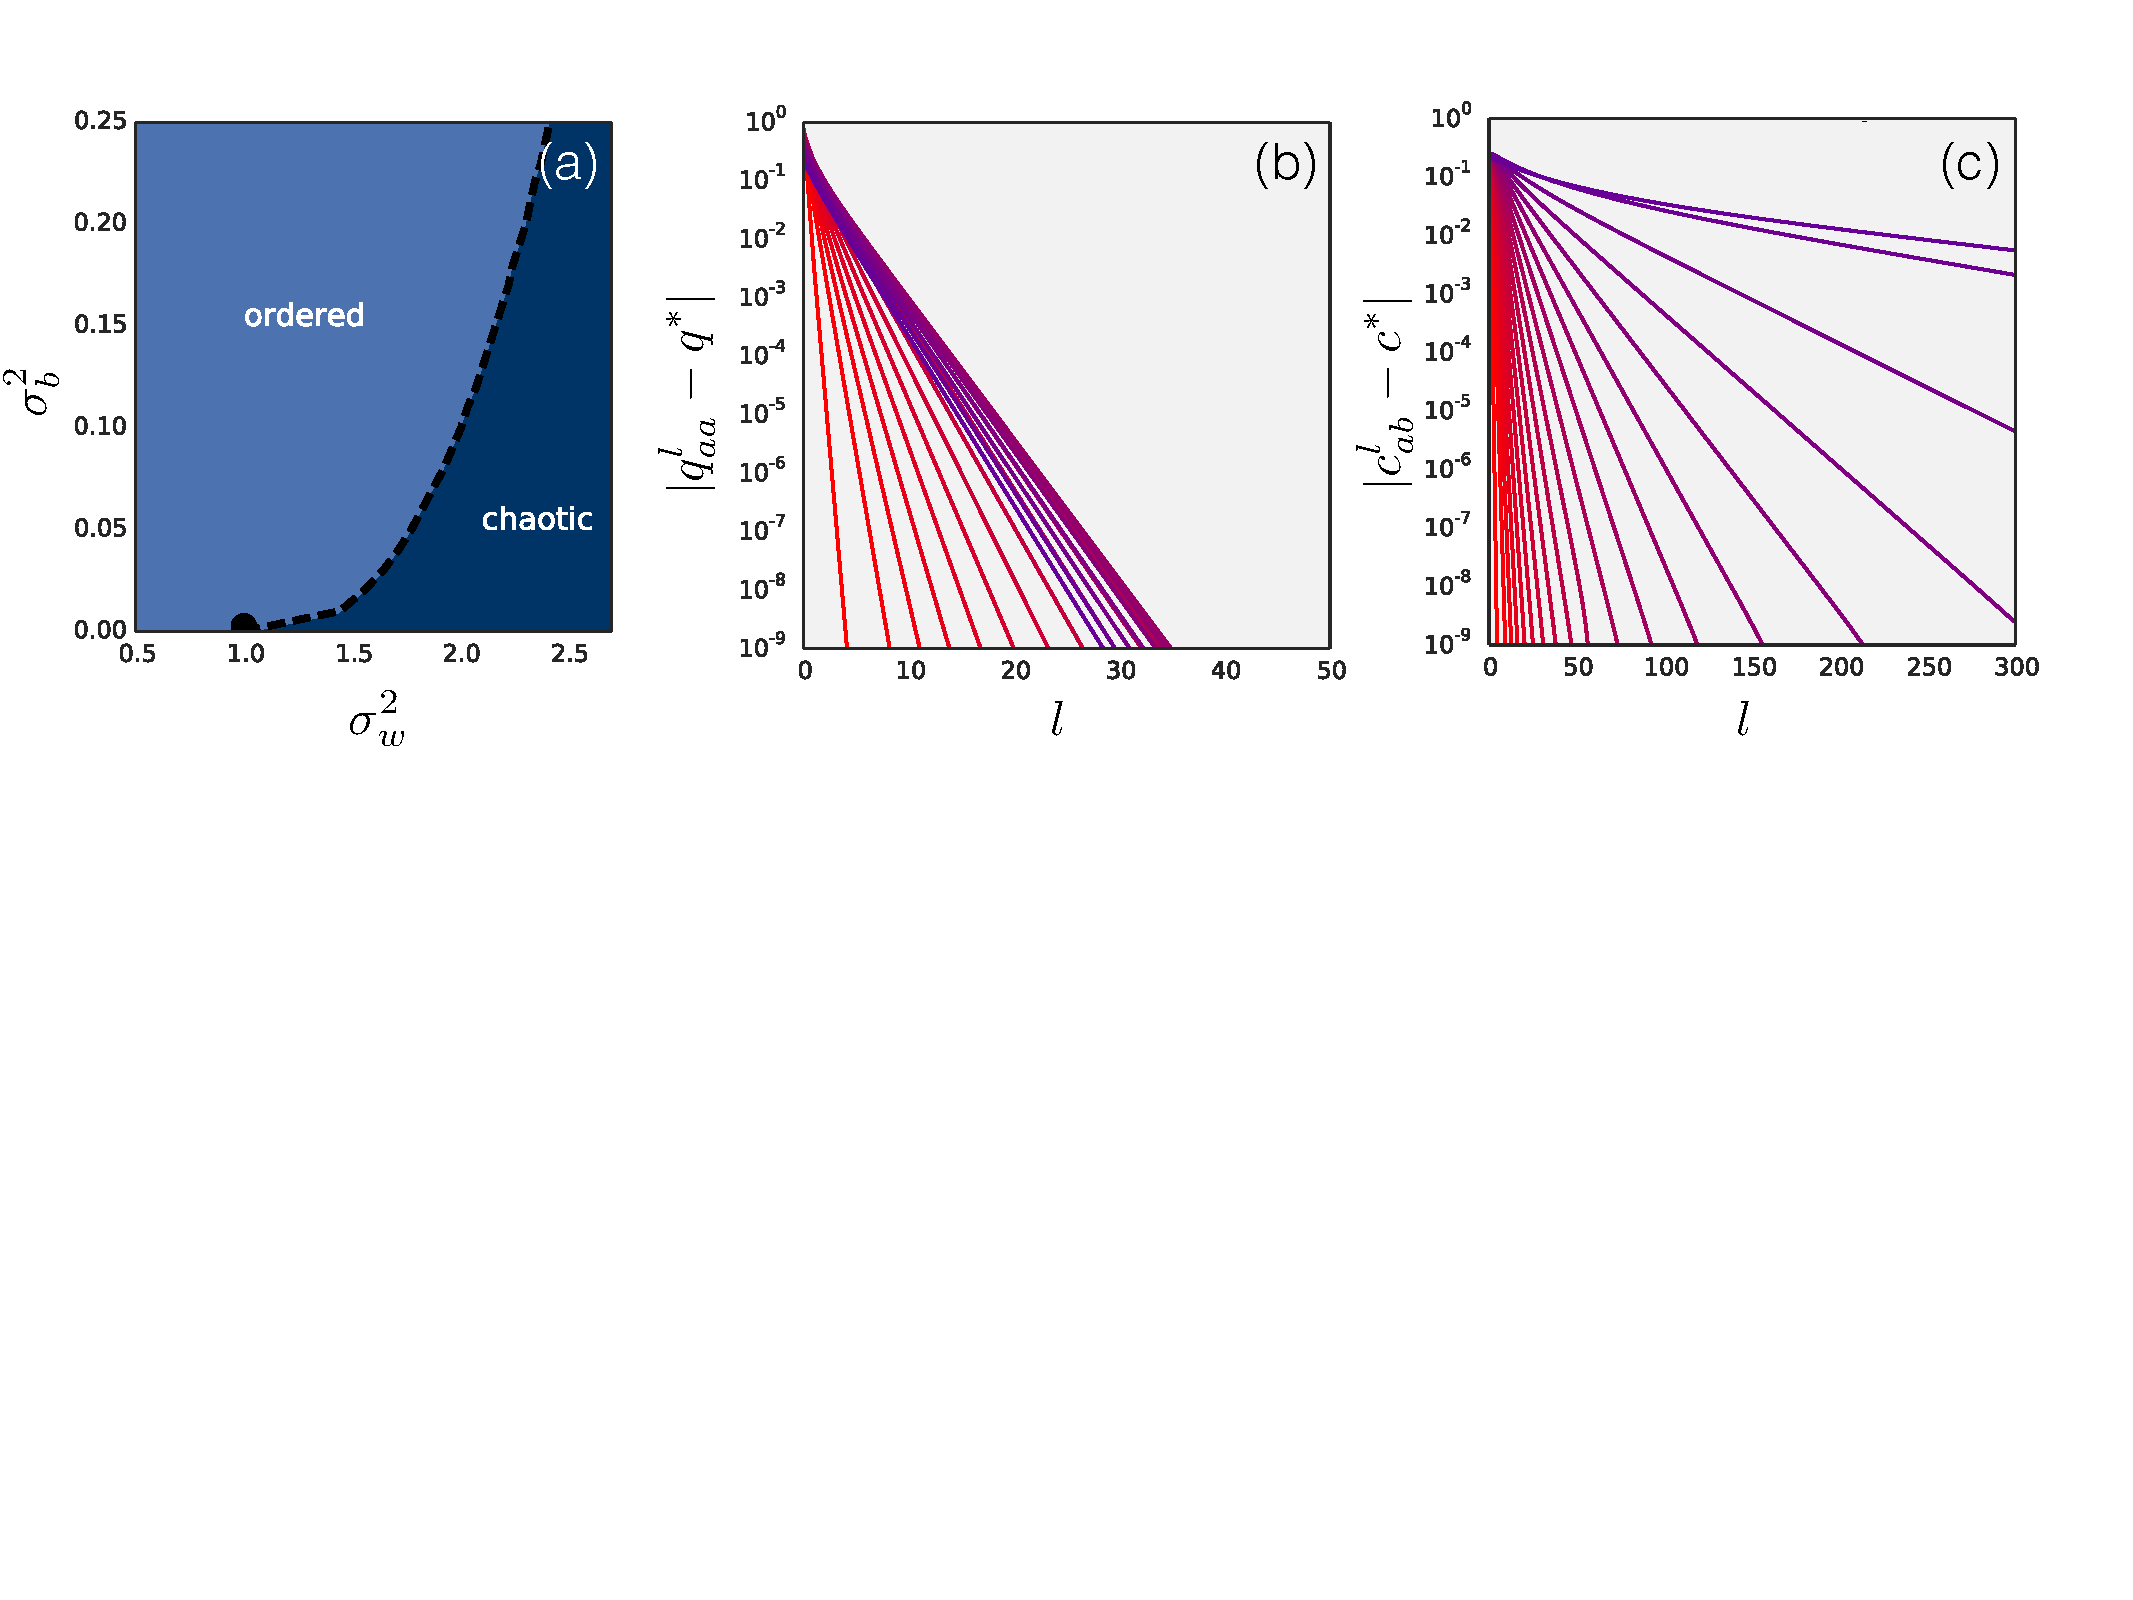
\includegraphics[width=\linewidth]{figures_julyan/bdl/figure_1}
\caption{(a) Edge of chaos diagram showing the boundary between ordered and chaotic phases as a function of $\sigma_w^2$ and $\sigma_b^2$. (b) The residual $|q^* - q_{aa}^l|$ as a function of depth on a log-scale with $\sigma_b^2 = 0.05$ and $\sigma_w^2$ from 0.01 (red) to 1.7 (purple). Clear exponential behavior is observed. (c) The residual $|c^* - c_{ab}^l|$ as a function of depth on a log-scale. Again, the exponential behavior is clear. The same color scheme is used here as in (b).  \label{fig:phase_diagram}}
\end{center}
\hfill\textcolor{gray}{From \citet{schoenholz2016deep}}
\end{figure}


\end{frame}


\subsection{Unit priors get heavier with depth}

\begin{frame}{Understanding priors at the unit level}
	\begin{definition}[Generalized Weibull-tail on $\mathbb{R}$]
\label{def:gen_weibull-tail_r}
A random variable $X$ is generalized Weibull-tail on $\mathbb{R}$ with tail parameter $\beta > 0$ if both its right and left tails are upper and lower bounded by some Weibull-tail functions with tail parameter~$\beta$:
\begin{align*}
    \edr^{-x^{\beta} l_1^r(x)} \le & \overline{F}_X(x) \le \edr^{-x^{\beta} l_2^r(x)}, \quad \ \ \ \text{for }x > 0 \text{ and $x$ large enough}, \\
    \edr^{-|x|^{\beta} l_1^l(|x|)} \le & F_X(x) \le \edr^{-|x|^{\beta} l_2^l(|x|)}, \quad \text{for } x < 0 \text{ and $-x$ large enough},
\end{align*}
where $l_1^r$, $l_2^r$, $l_1^l$ and $l_2^l$ are slowly-varying functions. 
We note $X \sim GWT(\beta)$. 
\end{definition}
\end{frame}

\begin{frame}{Understanding priors at the unit level}
This tail description reveals the difference between hidden units' distributional properties in finite- and infinite-width Bayesian neural networks, since 
hidden units are generalized Weibull-tail with a tail parameter depending on those of the weights:
\begin{theorem}[\citealp{vladimirova2021accurate}]
\label{theorem:hidden_units_are_gwt}
Consider a Bayesian neural network  with ReLU activation function. Let $\ell$-th layer weights be independent symmetric generalized Weibull-tail on~$\mathbb{R}$ with tail parameter $\beta^{(\ell)}_w$. 
Then conditional on the input $\bx$, the marginal prior distribution induced by forward propagation on any pre-activation is generalized Weibull-tail on~$\mathbb{R}$: for any $1\leq \ell\leq L$, and for any $1\leq m\leq H_\ell$,
$$g_m^{(\ell)}\sim GWT(\beta^{(\ell)}),$$
with tail parameter $\beta^{(\ell)}$ such that $\frac{1}{\beta^{(\ell)}} = \frac{1}{\beta^{(1)}_w} + \dots + \frac{1}{\beta^{(\ell)}_w}$,
where a $GWT$ distribution is defined in Definition~\ref{def:gen_weibull-tail_r}.
\end{theorem}
Note that the most popular case of weight prior, iid Gaussian \citep{neal1996bayesian}, corresponds to $\text{GWT}_{\mathbb{R}}(2)$ weights. This leads to units of layer $\ell$ which are $\text{GWT}_{\mathbb{R}}(\frac{2}{\ell})$. 
\end{frame}

\begin{frame}{Understanding priors at the unit level}


\def\bW{\boldsymbol{W}}
\def\bU{\boldsymbol{U}}
\def\Lnorm{\mathcal{L}}

\begin{center}
\begin{tabular}{@{}cclc@{}}
\toprule
Layer                         & Penalty on $\bW$         & \multicolumn{2}{c}{Approximate penalty on $\bU$}         \\ \toprule
$1$ & $\Vert \bW^{(1)}\Vert_2^{2}$, $\Lnorm^2$   & $\Vert \bU^{(1)}\Vert_2^{2}$ & $\Lnorm^2$  (weight decay)\\%\hline
$2$ & $\Vert \bW^{(2)}\Vert_2^{2}$, $\Lnorm^2$   & $\Vert \bU^{(2)}\Vert$ & $\Lnorm^1$  (Lasso)\\%\hline
% \vdots &\vdots &\vdots \\
$\ell$ & $\Vert \bW^{(\ell)}\Vert_2^{2}$, $\Lnorm^2$   & $\Vert \bU^{(\ell)}\Vert_{2/\ell}^{2/\ell}$ & $\Lnorm^{2/\ell}$ \\ 
% $\ell = L$ & $\Vert \bW^{(L)}\Vert_2^{2}$, $\Lnorm^2$   & $\Vert \bU^{(L)}\Vert_{2/L}^{2/L}$, $\Lnorm^{2/L}$ \\ 
\bottomrule
\end{tabular}\bigskip 

  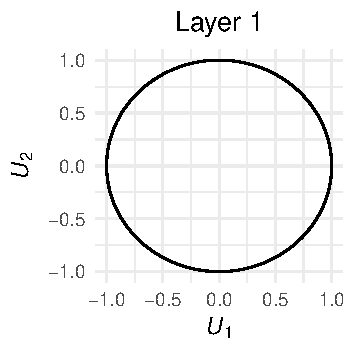
\includegraphics[width=.32\textwidth]{figures_julyan/bdl/001}
  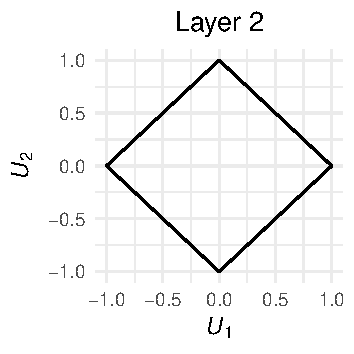
\includegraphics[width=.32\textwidth]{figures_julyan/bdl/002}
  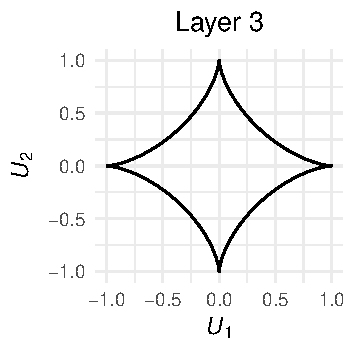
\includegraphics[width=.32\textwidth]{figures_julyan/bdl/003}

\end{center}

\end{frame}

\subsection{Other priors}



\begin{frame}{Other priors}
\begin{itemize}
	\item Although Gaussian priors are simple and widely used, they are not the only option. 
	\item For some applications, it is useful to use shrinkage or sparsity promoting priors which encourage most of the weights to be small/close to zero. Examples of such priors
	\begin{itemize}
	 \item  Laplace prior
	$$p_\lambda(x) = \frac{\lambda}{2}e^{-\lambda|x|}.$$
		\item spike-and-slab
	\end{itemize}
\end{itemize}

\end{frame}






%%%%%%%%%%%%%%%%%%%%%%%%%%%%%%%%%%%%%%%%%%%%%%%%%%%%%%%%
\section{Inference algorithms}
%%%%%%%%%%%%%%%%%%%%%%%%%%%%%%%%%%%%%%%%%%%%%%%%%%%%%%%%
\begin{frame}
	
\end{frame}

\begin{frame}{Bayesian inference: basic sampling algorithm}
Denote data by $D=\{D_x,D_y\}$ and parameters (weights) by $\boldsymbol{\theta}$.
\begin{center}
	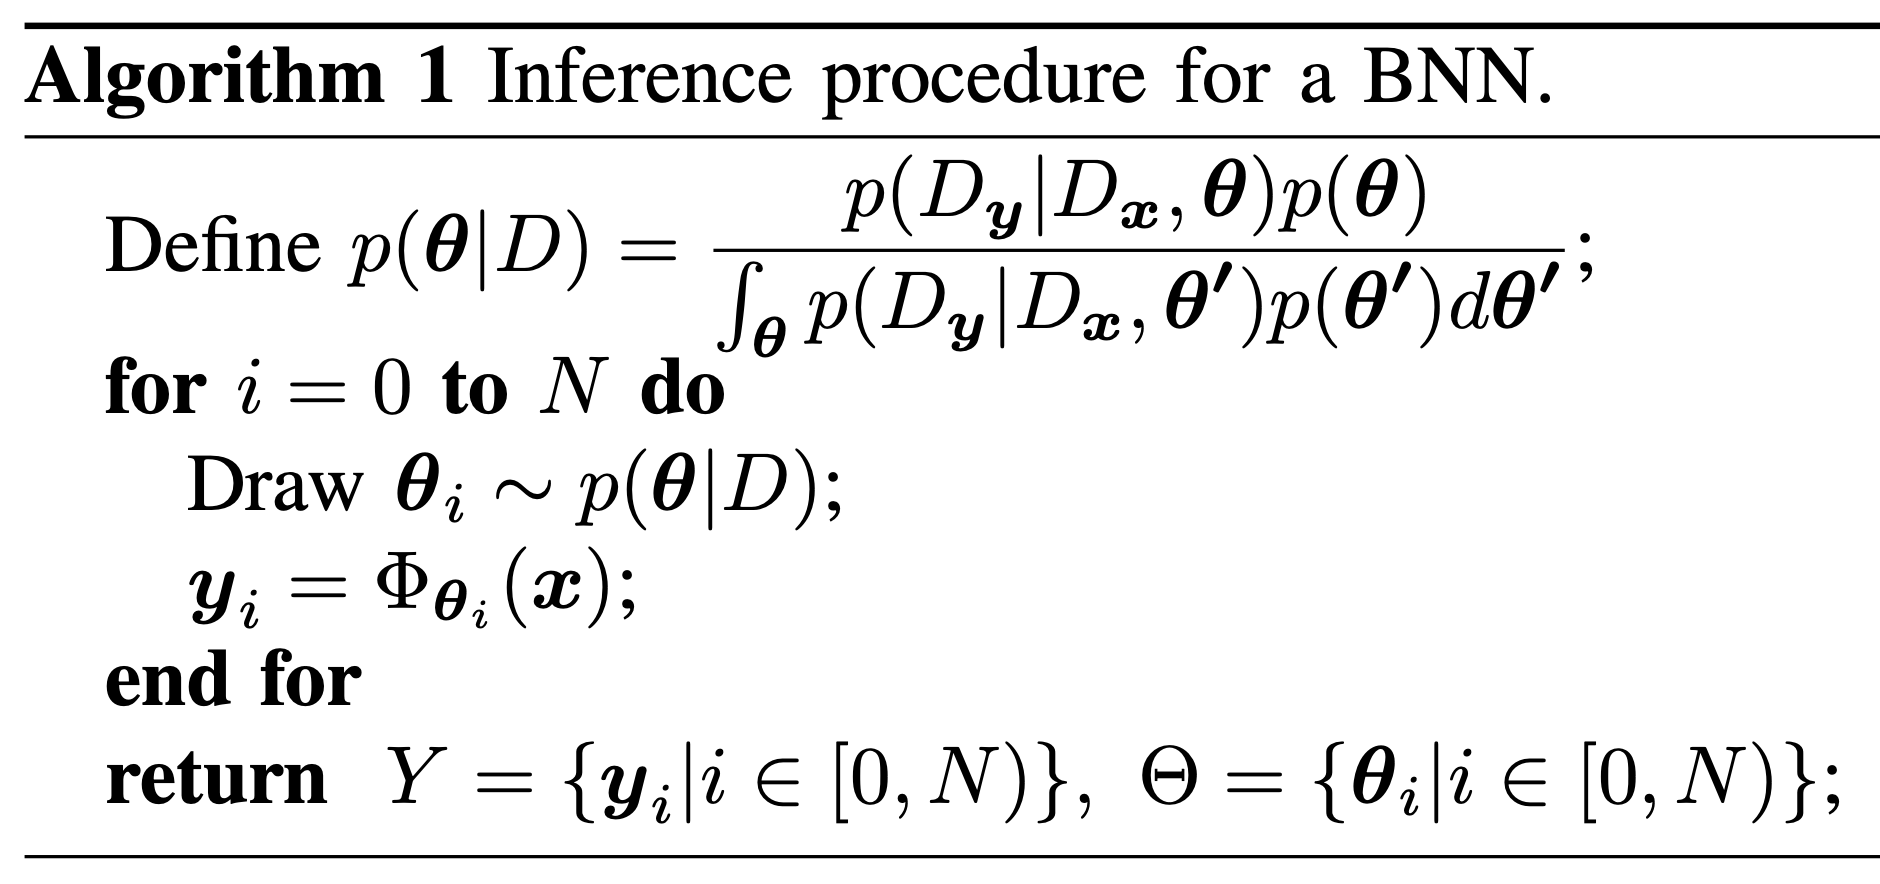
\includegraphics[width=.8\textwidth]{figures_julyan/bdl/hands-on/algo1}
\end{center}
\end{frame}



\begin{frame}{Laplace approximation}
Computes a Gaussian approximation to the posterior centered at the MAP estimate

\begin{itemize}
	\item It is simple
	\item But... computing the Hessian is expensive, and may result in a non-positive definite matrix since the log likelihood of deep neural networks is non-convex.
	\item Gauss--Newton approximation to the Hessian
\end{itemize}

\begin{block}{Generalized Gauss--Newton approximation}
	$$\bH^{\mathrm{GGN}}:= \sum_{i=1}^n \mathcal{J}_{\bw}(\bx_i)^{\top}\boldsymbol{\Lambda}(\by_i;f_i)\mathcal{J}_{\bw}(\bx_i),$$
where $\mathcal{J}_{\bw}(\bx)$ is the network per-sample Jacobian $\left[\mathcal{J}_{\bw}(\bx)\right]_{c}=\nabla_{\bw}f_c(\bx;\bw_{\hat{\rho}})$, and $\boldsymbol{\Lambda}(\by;f)=-\nabla^2_{ff}\log p(\by;f)$ is the per-input noise matrix.% \citep{kunstner2019limitations}.
\end{block}

\end{frame}




\begin{frame}{Bayesian neural networks: early algorithms}
\begin{itemize}[<+->]
	\item \alert{Markov chain Monte Carlo} (MCMC), \alert{Hamiltonian Monte Carlo} (HMC). No-U-Turn sampler (NUTS) it most often used in probabilistic programming languages (Stan, PyMC3, Pyro, etc): is improves over classic HMC by allowing hyperparameters to be set automatically instead of manually
	\item \alert{Variational inference} (VI): scales better than MCMC algorithms. Idea: find an approximate variational distribution in a variational family that is as close as possible to the exact posterior by minimizing the Kullback--Leibler divergence. Turns sampling into optimization.
	\item \alert{Stochastic variational inference} (SVI): scales better than VI, stochastic gradient descent method applied to VI. Gradient of objective is computed only on mini-batches.
\end{itemize}
\end{frame}




\begin{frame}{Bayesian neural networks: early algorithms}
\begin{alertblock}{BUT}
	Stochasticity in gradient estimation stops backpropagation from functioning
\end{alertblock}
\pause


\begin{block}{Tricks for Monte Carlo gradient estimation}
	A number of \alert{tricks} \citep[see][]{mohamed2020montecarlo}
	\begin{itemize}
		\item Log-derivative trick: score function estimators
		\item Reparameterisation trick: pathwise derivative estimator
		\item Measure-valued gradient estimators
	\end{itemize}
\end{block}
\end{frame}



\begin{frame}{Bayesian neural networks: adapted algorithms}
\begin{itemize}
	\item \alert{Bayes-by-backprop} (BBB) and \alert{probabilistic backpropagation} (PBP): implement the reparameterisation trick
	\item \alert{Monte Carlo dropout}: turning dropout into an approximate Bayesian algorithm (variational inference)
	\item  \alert{Bayes via stochastic gradient descent}: includes MCMC algorithms based on the SGD dynamic such as stochastic gradient Langevin dynamic (SGLD) and Variational Inference based on SGD dynamic such as ensembling
\end{itemize}
\end{frame}


\begin{frame}[allowframebreaks]{Monte Carlo dropout}
Dropout technique reinterpreted as a form of approximate Bayesian variational inference \citep{kingma2015variational,gal2016dropout}.

\alert{Idea}: performing random sampling at test time. Instead of turning off the dropout layers at test time (as is usually done), \textcolor{orange2}{hidden units} are randomly dropped out according to a \textcolor{orange2}{Bernoulli$(p)$} distribution. Repeating this operation $M$ times provides $M$ versions of the MAP estimate of the network parameters $\bw^m$, $m=1,\ldots,M$ (where some units of the MAP are dropped), yielding an approximate posterior predictive in the form of the equal-weight average:
\begin{equation*}
%\label{eq:MCdropout_post_pred}
	p(y\vert x, \mathcal{D}^n)\approx \frac{1}{M}\sum_{m=1}^M p(y\vert x, \bw^m).
\end{equation*}

\vfill 

\begin{itemize}
	\item Monte Carlo dropout captures some uncertainty from out-of-distribution (OOD) inputs
	\item But... \alert{does not provide valid posterior uncertainty}
	\item \citet{folgoc2021mc} show that the Monte Carlo dropout posterior predictive assigns \alert{zero probability} to the true model posterior predictive distribution
\end{itemize}
\end{frame}


\begin{frame}{Tempered and cold posteriors}
\begin{block}{Tempered posterior}
	A \alert{tempered posterior distribution} with \alert{temperature parameter} $\alert{T}>0$ is defined as $$p(\bw|D) \propto \exp(U (\bw)/\alert{T} )$$ where $U(\bw)$ is the posterior energy function
\begin{equation*}
 U(\bw) :=  \log p(\mathcal{D} | \bw) + \log p(\bw),
\end{equation*}
\end{block}

\pause

\begin{block}{Cold posterior effect}
Empirical evidence \citep{wenzel2020good} that posteriors  exponentiated to some power greater than one (or, equivalently, dividing the energy function $U(\bw)$ by some temperature $T<1$), \alert{performs better} than an untempered one.
\end{block}



\end{frame}



%%%%%%%%%%%%%%%%%%%%%%%%%%%%%%%%%%%%%%%%%%%%%%%%%%%%%%%%
\section{Performance metrics}
%%%%%%%%%%%%%%%%%%%%%%%%%%%%%%%%%%%%%%%%%%%%%%%%%%%%%%%%


\begin{frame}{Performance metrics}
\begin{itemize}
	\item \alert{Predictive performance}: ability of the model to give correct answers. Based on metrics, eg: mean square error, risk of 0-1 loss for classification task.
	\item \alert{Model calibration}: assessing that the network is neither overconfident nor underconfident about its prediction. Requires using a test set. Eg: expected calibration error (ECE).
\end{itemize}
\end{frame}


\section*{References}
\setbeamertemplate{bibliography item}[text]%,
\begin{frame}[allowframebreaks]
\frametitle{References}
\small
\printbibliography
\normalsize
\end{frame}
\end{document}
